\documentclass[10pt,conference]{IEEEtran}
%%\settopmatter{printacmref=false} % Removes citation information below abstract
%%\renewcommand\footnotetextcopyrightpermission[1]{} % removes footnote with conference information in first column
\pagestyle{plain} % removes running headers
\usepackage{amsmath}
\usepackage{xcolor}
\usepackage{booktabs} % For formal tables
\usepackage{listings}
\usepackage{caption}
\usepackage{subcaption}
\usepackage[ruled,linesnumbered]{algorithm2e}
\lstset{escapeinside={<@}{@>}}
\usepackage{url}
\def\BibTeX{{\rm B\kern-.05em{\sc i\kern-.025em b}\kern-.08em
		T\kern-.1667em\lower.7ex\hbox{E}\kern-.125emX}}


%% The acronym package provides support for defining acronyms, providing
%% their expansion when first used, and building glossaries.  See the
%% example in glossary.tex and the example usage throughout the example
%% document.
%% NOTE: to use \MakeTextLowercase with acsfont
%%   we *must* use the `nohyperlinks' option -- it causes errors with
%%   hyperref otherwise.  See Section 5.2 in the ``LaTeX 2e for Class
%%   and Package Writers Guide'' (clsguide.pdf) for details.
\usepackage{hyperref}
\usepackage[printonlyused,nohyperlinks]{acronym}

\acrodef{xhr}[XHR]{{\tt XMLHttpRequest}}
\acrodef{WAF}[WAF]{Web Application Firewall}
\acrodef{XSS}[XSS]{Cross-Site Scripting}
\acrodef{CSRF}[CSRF]{Cross-Site Request Forgery}
\acrodef{CSP}[CSP]{Content Security Policy}
\acrodef{CVE}[CVE]{Common Vulnerability and Exposures}
\acrodef{DDoS}[DDoS]{Distributed Denial-of-Service}
\acrodef{SQL}[SQL]{Structured Query Language}
\acrodef{CMS}[CMS]{Content Management System}
\acrodef{PoC}[PoC]{proof of concept}

\definecolor{lightgray}{rgb}{.9,.9,.9}
\definecolor{darkgray}{rgb}{.4,.4,.4}
\definecolor{purple}{rgb}{0.65, 0.12, 0.82}
\lstdefinelanguage{JavaScript}{
  keywords={typeof, new, true, false, catch, function, return, null, catch, switch, var, if, in, while, do, else, case, break},
  keywordstyle=\color{black}\bfseries,
  ndkeywords={export, boolean, throw, implements, import, this}, % removed class because of clash in html
  ndkeywordstyle=\color{darkgray}\bfseries,
  identifierstyle=\color{black},
  sensitive=false,
  comment=[l]{//},
  morecomment=[s]{/*}{*/},
  commentstyle=\color{black}\ttfamily,
  stringstyle=\color{black}\ttfamily,
  morestring=[b]',
  morestring=[b]"
}
\lstset{
   %language=JavaScript,
   %backgroundcolor=\color{lightgray},
   extendedchars=true,
   basicstyle=\footnotesize\ttfamily,
   showstringspaces=false,
   showspaces=false,
   %numbers=left,
   numberstyle=\footnotesize,
   numbersep=9pt,
   tabsize=2,
   breaklines=true,
   breakatwhitespace=true,
   showtabs=false,
   captionpos=t
}

%%
%% Macros
\newcommand{\sys}[0]{XSnare\xspace}
\newcommand{\xss}[0]{\ac{XSS}\xspace}
\newcommand{\xhr}[0]{\ac{xhr}\xspace}
\newcommand{\js}[1]{\lstinline[mathescape,basicstyle=\normalsize]^#1^}
\newcommand{\code}[1]{\lstinline[mathescape,basicstyle=\normalsize]^#1^}

% \usepackage{ifthen}
% \usepackage[normalem]{ulem} % for \sout
% \usepackage{amssymb}

% \newcommand{\ra}{$\rightarrow$}
% \newboolean{showedits}
% %\setboolean{showedits}{true} % toggle to show or hide edits
% \ifthenelse{\boolean{showedits}}
% {
% 	\newcommand{\ugh}[1]{\textcolor{red}{\uwave{#1}}} % please rephrase
% 	\newcommand{\ins}[1]{\textcolor{blue}{\uline{#1}}} % please insert
% 	\newcommand{\del}[1]{\textcolor{red}{\sout{#1}}} % please delete
% 	\newcommand{\chg}[2]{\textcolor{red}{\sout{#1}}{\ra}\textcolor{blue}{\uline{#2}}} % please change
% }{
% 	\newcommand{\ugh}[1]{#1} % please rephrase
% 	\newcommand{\ins}[1]{#1} % please insert
% 	\newcommand{\del}[1]{} % please delete
% 	\newcommand{\chg}[2]{#2}
% }

% \newboolean{showcomments}
% \setboolean{showcomments}{false}
% % \setboolean{showcomments}{true}
% \newcommand{\id}[1]{$-$Id: scgPaper.tex 32478 2010-04-29 09:11:32Z oscar $-$}
% \newcommand{\yellowbox}[1]{\fcolorbox{gray}{yellow}{\bfseries\sffamily\scriptsize#1}}
% \newcommand{\triangles}[1]{{\sf\small$\blacktriangleright$\textit{#1}$\blacktriangleleft$}}
% \ifthenelse{\boolean{showcomments}}
% %{\newcommand{\nb}[2]{{\yellowbox{#1}\triangles{#2}}}
% {\newcommand{\nbc}[3]{
%  {\colorbox{#3}{\bfseries\sffamily\scriptsize\textcolor{white}{#1}}}
%  {\textcolor{#3}{\sf\small$\blacktriangleright$\textit{#2}$\blacktriangleleft$}}}
%  \newcommand{\version}{\emph{\scriptsize\id}}}
% {\newcommand{\nbc}[3]{}
%  \renewcommand{\ugh}[1]{#1} % please rephrase
%  \renewcommand{\ins}[1]{#1} % please insert
%  \renewcommand{\del}[1]{} % please delete
%  \renewcommand{\chg}[2]{#2} % please change
%  \newcommand{\version}{}}
% \newcommand{\nb}[2]{\nbc{#1}{#2}{orange}}


% \usepackage{wasysym}
% \newcommand\yesml[1]{\nbc{ML {\textcolor{yellow}\sun}}{#1}{mircolor}}


%% \usepackage{algorithm}
%% \usepackage[noend]{algpseudocode}
\usepackage{xspace}
\usepackage{tikz}
\usepackage{array}
%\usepackage{amsmath,amssymb}
\usepackage{xcolor}


\newcommand{\algformat}[1]{\textsc{#1}\xspace}
\newcommand{\netsolver}{\algformat{Net\-solver}}
\newcommand{\monosat}{\algformat{Mono\-SAT}}
\def\checkmark{\tikz\fill[scale=0.4](0,.35) -- (.25,0) -- (1,.7) -- (.25,.15) -- cycle;}
\newcommand{\eg}{\emph{e.g.,}\xspace}
\newcommand{\ie}{\emph{i.e.,}\xspace}

\newcolumntype{C}[1]{>{\centering\let\newline\\\arraybackslash}m{#1}}

\newcommand{\true}{\textsc{True}\xspace}
%\newcommand{\comment}[1]{}

\newboolean{showcomments}


% \setboolean{showcomments}{false}
\setboolean{showcomments}{true}


\ifthenelse{\boolean{showcomments}}
{\newcommand{\nbc}[3]{
 {\colorbox{#3}{\bfseries\sffamily\scriptsize\textcolor{white}{#1}}}
 {\textcolor{#3}{\sf\small$\blacktriangleright$\textit{#2}$\blacktriangleleft$}}}
}{\newcommand{\nbc}[3]{} 
 \newcommand{\version}{}}
\newcommand{\nb}[2]{\nbc{#1}{#2}{orange}}


\definecolor{ibcolor}{rgb}{0.4,0.6,0.2}
\definecolor{hhcolor}{rgb}{0.2,0.6,0.6}
\definecolor{nkcolor}{rgb}{0.8,0.5,0.3}
\definecolor{sbcolor}{rgb}{0.0,0.0,1}
\newcommand\iv[1]{\nbc{IB}{#1}{ibcolor}}
\newcommand\hh[1]{\nbc{HH}{#1}{hhcolor}}
\newcommand\nk[1]{\nbc{NK}{#1}{nkcolor}}
\newcommand\ijcai[1]{\nbc{IJCAI+}{#1}{nkcolor}}
\newcommand\aij[1]{\nbc{AIJ+}{#1}{sbcolor}}
\newcommand\sam[1]{\nbc{SB}{#1}{sbcolor}}

\definecolor{todocolor}{rgb}{0.9,0.1,0.1}
\newcommand\todo[1]{\nbc{TODO}{#1}{todocolor}}


%% The following commands causes chapter and section references to
%% uppercase the part name.
\renewcommand{\chapterautorefname}{Chapter}
\renewcommand{\sectionautorefname}{Section}
\renewcommand{\subsectionautorefname}{Section}
\renewcommand{\subsubsectionautorefname}{Section}
\renewcommand{\algorithmautorefname}{Algorithm}


%%%%%%%%%%%%%%% URLs with special characters
% from: https://tex.stackexchange.com/questions/250102/insert-special-symbols-in-url
\urldef{\deprecatexssauditorURL}\url{https://groups.google.com/a/chromium.org/forum/#!msg/blink-dev/TuYw-EZhO9g/blGViehIAwAJ}

%%%%%%%%%%%%%%%

	
\begin{document}
	\title{\sys: Application-specific client-side cross-site scripting protection}
	
	
	\author{\IEEEauthorblockN{Anonymous author(s)}
	}
	
%%%%%%%%%%%%%%%%%%%%%%%%%%%%%%%%%%%%%%%%%%%%%%%%%%%%%%%%%%
%%%%%%%%%%%%%%%%%%%%%%%%%%%%%%%%%%%%%%%%%%%%%%%%%%%%%%%%%%

	%\author{\IEEEauthorblockN{Jos\'e Carlos Pazos}
	%	\IEEEauthorblockA{\textit{Department of Computer Science} \\
	%		\textit{University of British Columbia}\\
	%		Vancouver, Canada \\
	%		jpazos@cs.ubc.ca}
	%	\and
	%	\IEEEauthorblockN{Jean-S\'ebastien L\'egar\'e}
	%	\IEEEauthorblockA{\textit{Department of Computer Science} \\
	%		\textit{University of British Columbia}\\
	%		Vancouver, Canada \\
	%		jslegare@cs.ubc.ca}
	%	\and
	%	\IEEEauthorblockN{William Aiello}
	%	\IEEEauthorblockA{\textit{Department of Computer Science} \\
	%			\textit{University of British Columbia}\\
	%			Vancouver, Canada \\
	%			aiello@cs.ubc.ca}
	%	\and
	%	\IEEEauthorblockN{Ivan Beschastnikh}
	%	\IEEEauthorblockA{\textit{Department of Computer Science} \\
	%		\textit{University of British Columbia}\\
	%		Vancouver, Canada \\
	%		bestchai@cs.ubc.ca}
	%}
	
%%%%%%%%%%%%%%%%%%%%%%%%%%%%%%%%%%%%%%%%%%%%%%%%%%%%%%%%%%
%%%%%%%%%%%%%%%%%%%%%%%%%%%%%%%%%%%%%%%%%%%%%%%%%%%%%%%%%%
	
	
	\maketitle
	\begin{abstract}

We present \sys, a fully client-side \ac{XSS}
solution, implemented as a Firefox extension. Our approach takes
advantage of available previous knowledge of a web application's
HTML template content, as well as the rich context available in the
DOM to block XSS attacks. It uses a database of exploit
descriptions, which are written with the help of previously recorded
CVEs, to prevent them. CVEs for XSS are widely available and are
one of the main ways to tackle zero-day exploits. We effectively
single out potential injection points for exploits in the HTML and sanitize content to prevent malicious payloads from appearing in the DOM.

XSnare is a framework for emulating server-side software sanitization on the application client-side. It can protect application users before application developers release patches and before server operators apply them.

We evaluate the applicability of our approach by studying
104 recent CVEs related to XSS attacks, and find that our tool
defends against 93.75\% of these exploits. To the best of our knowledge,
our work is the first to provide a protection mechanism for XSS that is
application specific, and based on publicly available CVE information.
We show that XSnare's specificity protects users against exploits which evade other, more generic, anti-XSS approaches.

Our performance evaluation shows that our extension's overhead on web page loading time is less than 10\% for 72.6\% of the sites studied.

\end{abstract}

	\acresetall	% reset all acronyms used so far
	
	% assume we've used these common acronyms already
	% this will prevent their expansion
	% \acused{XSS}
	\acused{CVE}
	\acused{SQL}
	\acused{DDoS}
	
	\section{Introduction} \label{introduction}

\ac{XSS} is still one of the most dominant web
vulnerabilites. In 2017, a report showed that 50\% of websites
contained at least one \ac{XSS} vulnerability~\cite{Acunetix}. Countermeasures
exist, but many of them lack widespread deployment, and so have been unable to protect users.
Many of these defenses require server-side and browser modifications~\cite{Jim:2007:DSI:1242572.1242654,Nadji:2009,Wurzinger:2009:SMX:1656360.1656379,10.1007/978-3-642-31540-4_17} and/or additional front-end developer effort~\cite{10.1007/978-3-319-66399-9_7}. Still, others disable client-side
functionality~\cite{Noscript,Snyder:2017:MWD:3133956.3133966},
sometimes rendering websites unusable. We believe many of these
solutions have not seen widespread adoption because they simply are
not practical: developers might not be willing, or might not have the
resources or expertise available to implement them. Furthermore, even
when software patches are available, many website
administrators won't apply updates immediately: a 2016 study found that
61\% of WordPress websites were running a version with known security
vulnerabilities~\cite{Sucuri}, and another found that 30.95\% of
Alexa's top 1 Million sites run a vulnerable version of WordPress~\cite{wpwhitesecurity}.
As the number of websites using client-side
technologies continues to increase (a study showed that as early as
2012, almost 100\% of the Alexa top 500 sites were using
JavaScript~\cite{Stock:2017:WTI:3241189.3241265}), users are effectively left at
the mercy of developers and administrators if they wish to browse the
web safely.


\begin{figure}[h]
  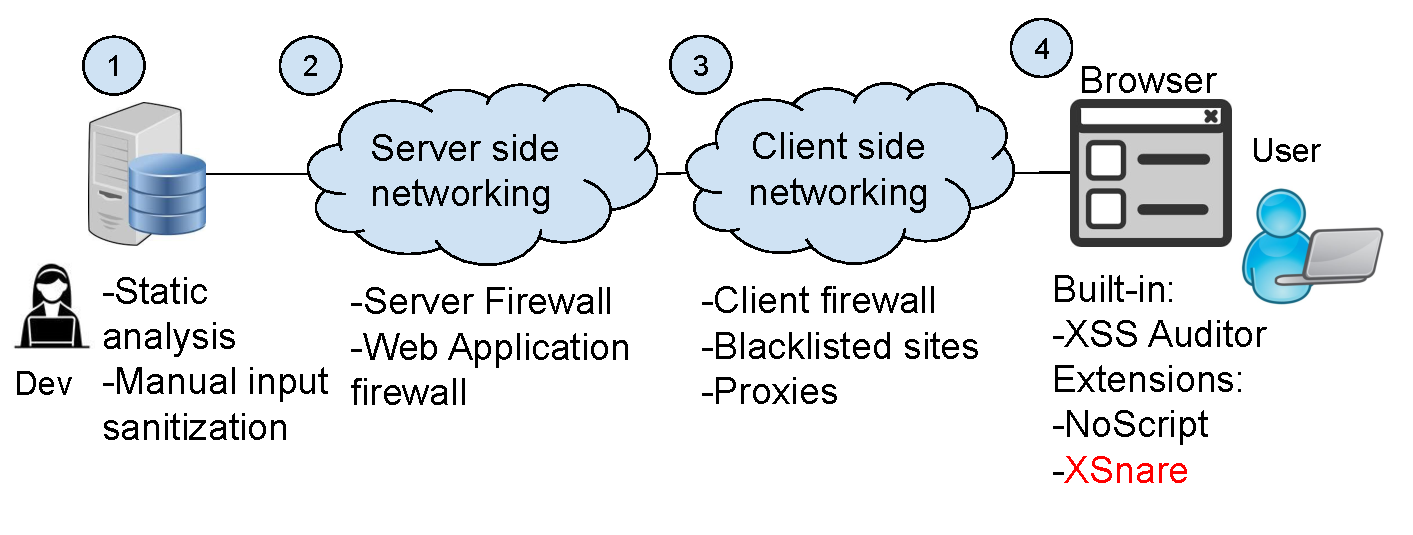
\includegraphics[scale=0.37]{img/web_app_architecture_one.pdf}
  \vspace*{-5.0ex}
  \caption{Architecture of typical web applications. Different security solutions apply at distinct layers.}
  \label{fig:web_architecture}
\end{figure}

Vulnerability defences can be implemented in multiple layers of the web application stack (Figure~\ref{fig:web_architecture}). Each layer opens different defence options:
%Further details of these different approaches are described in Section 5:
\begin{enumerate}
	\item At the application's server-side, the developer is
          trying to defend herself against malicious users. The first
          line of defence from these vulnerabilities lies in the
          application logic itself. The developer might choose to
          ensure safety of the code, either by using third-party
          solutions, or by securing the code themselves, for example,
          by applying static analysis on the server code to detect
          unsanitised input.
	\item In the hosting environment, developers deploy
          defences including generic firewalls and more specific \acp{WAF}, which defend against attacks
          such as \ac{DDoS}, \ac{SQL} injections and \ac{XSS}.
	\item In the client's environment, the user requires protection from
          malicious websites, and may install their own network firewall,
          network filters, and web proxies.
	\item The last line of defence is the browser. \sys operates at this point.
          The browser has built-in defences, such as
          Chrome's \ac{XSS} Auditor~\cite{xssauditor}. But the user can also
          install third-party extensions to block malicious requests and
          responses. % such as the NoScript~\cite{Noscript} extension.
\end{enumerate}

Many of these approaches are either unfit for widespread deployment or
do not benefit from an application's contextual knowledge. For
example, a \ac{WAF} might be enough to defend against most \ac{XSS} attacks on
one deployment, but it would require each individual developer to have
the necessary knowledge and resources to integrate one. A network
proxy at the client-side will usually have a generic set of rules to
apply on incoming network traffic, and this will often lead to an
elevated rate of false positives. Browser built-in defences are very
coarse, and will only work on a subset of exploits. Chrome's XSS
Auditor, for example, only attempts to defend against reflected
\ac{XSS}. In fact, Google has recently announced its intention to deprecate
XSS Auditor, with reasons including "Bypasses abound", "It prevents
some legit sites from working", and "Once detected, there’s nothing
good to do"~\cite{deprecatexssauditor}. Stock et
al.~\cite{Stock:2017:WTI:3241189.3241265} propose enhancements to the
XSS Auditor. Their work covers a wider range of exploits than the
auditor, but is limited to DOM-based \ac{XSS}. Our work is not particular
to a type of \ac{XSS}.

While there is much work in the server-side area,
\cite{Xu:2006:TPE:1267336.1267345,DBLP:conf/sec/Nguyen-TuongGGSE05,Pietraszek:2005:DAI:2146257.2146267,Bisht:2008:XPD:1428322.1428325}
(TODO: references for static analysis of php code for security), the
adoption of server-side techniques might not be feasible for many
developers. A 2018 study found that the average time to patch a \ac{CVE}
regardless of severity is 38 days, increasing to as much as 54 days
for low severity vulnerabilities, and the oldest unpatched \ac{CVE} was 340
days old~\cite{Rapid7}. A client-side solution does not rely on
application developers, so it ideally reduces the turnaround time
between a vulnerability and its patch. Furthermore, it is
complementary to the aforementioned techniques: a \ac{WAF} will not reduce
the security of a client-side approach by any means, and having these
two work in tandem is beneficial to the user's experience.

To provide users with the means to protect themselves in the absence
of control over servers, we strongly believe a novel client-side
solution must be delivered. A number of existing solutions in this
area also suffer from a high rate of false-positives and
false-negatives, due to the lack of information available at the
layers they operate at. For example, NoScript \cite{Noscript} works via domain
whitelisting, thus by default, JavaScript scripts and other code will
not execute. However, not all scripts outside of the whitelist should
be assumed to be malicious. Browser-level filters like XSS Auditor
work based on general policies and can therefore incorrectly sanitize
non-malicious content.

In contrast, we posit that the DOM is the right place to interpose for
the purpose of mitigating against these attacks, since we have the
full picture at that point. While most of the functionality we provide
could be done by a network filter on top of the browser, we require
some additional context to perform effective \ac{XSS} identification. In
particular, when an exploit manifests itself through dynamic
behaviour, like a network request initiated by an user's click, we
require knowledge of the tab which initiated the request to filter the
response. Previous work on client-side solutions has focused on
generic approaches to vulnerability detection
\cite{Kirda:2009:CCS:2639535.2639808,Jim:2007:DSI:1242572.1242654,Hallaraker:2005:DMJ:1078029.1078861}. Our
work is application-specific and can therefore be more precise when
targeting vulnerabilities.

Commonly, bug bounty hunters and penetration testers will scour
websites to find vulnerabilities and alert developers of issues in
these, as well as potential fixes. Developers will then fix the bugs
accordingly so that users are not subject to vulnerabilities. Inspired
by this workflow, we believe this process can be partly automated
using a firewall-based approach, so that users don't have to wait for
developers to update their code. A similar approach is presented in \cite{Kirda:2009:CCS:2639535.2639808}, as a client-side firewall-based 
network proxy. Rules dictate the links which can be accessed by a website
when generating requests, and can be created both automatically and manually
by an user. Contrary to our work, this technique does not protect against
attacks which do not generate a network request, such as deleting local
files. Furthermore, they rely on websites having a small amount of external
dynamic links to third-parties. This likely does not hold true anymore, 
as websites require an ever-increasing amount of dynamic content, with 
several interconnections with third-parties, such as advertisement, analytics,
and other user interactions.

Our system consists of three main components: a trusted Firefox
extension for interposing between the application and the DOM, a
periodically updated local database which maintains exploit
definitions and descriptions of the vulnerabilities to be targeted by
the extension in the form of signatures, and finally, a declarative
language for describing exploits, expressive enough for an user to be
precise about which parts of the HTML are vulnerable and how to
sanitize them.

We aim to reproduce the developer's intended server-side patch on the
client-side, therefore, we need to be able to determine the separation
between dynamic content and the static template, and pass the dynamic
elements to a sanitization function. We provide further details of the
mechanisms we provide to achieve this goal in Section
\ref{xsnare_design}.

We evaluate our application-specific, signature-based approach, by
testing it against recent \ac{XSS} CVEs. CVE databases are well-maintained
and widely available. They are one of the main tools used by
developers to patch their code against known vulnerabilities. 


To the
best of our knowledge, our work is the first to evaluate an \ac{XSS}
protection tool against real world exploits of this form at the scope
we do.



	\section{\sys Design} \label{xsnare_design}

 \begin{figure}[h]
	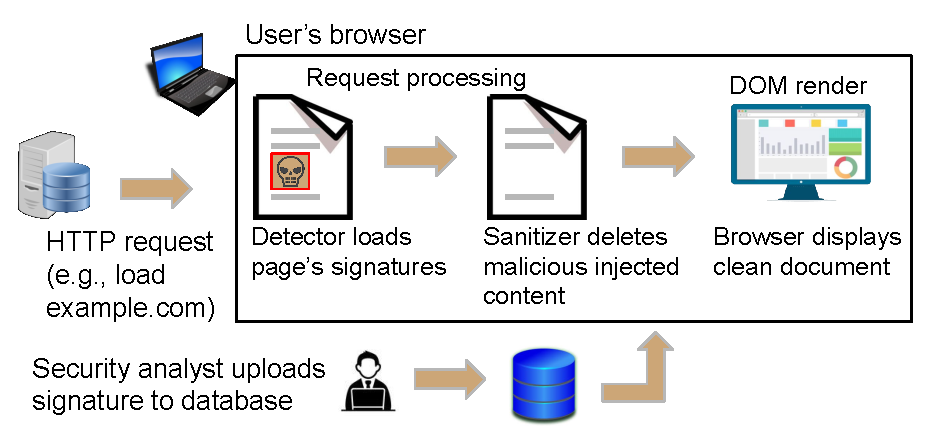
\includegraphics[scale=0.55]{img/xsnare.pdf}
	\caption{\sys's approach to protect against XSS.}
	\label{fig:xsnare}
\end{figure}

We now present the design of \sys and its components. % and how they interact with each other.
%
% \subsection{Operation, at a glance} \label{operation}
%
We begin with a high-level view of its operation (see
\autoref{fig:xsnare}): A user requests a page, \url{example.com}, on a
browser with the \sys extension installed.
%
The response may or may not contain
malicious \xss payloads.
%
Before the browser renders the document, \sys analyzes
the potentially malicious document. The extension loads signatures
from its local database into its detector. The detector analyzes the
HTML string arriving from the network, and identifies the signatures
which apply to the document. These signatures specify one or more
``injection spots'' in the document, which correspond, roughly
speaking, to regions of the DOM where improperly sanitized content
could be injected.  The extension's sanitizer
eliminates any malicious content and outputs a clean HTML document to
the browser for rendering (\autoref{filter_algorithm}).

%% The network filter is presented in \autoref{filter_algorithm} describes the
%% network filtering process. Section \ref{implementation} explains this
%% algorithm in more detail.

\subsection{An example application of \sys} \label{motivating_example}

To further explain our approach, we present a small example of how
DOM context can be used to defend against XSS, taken from CVE
2018-10309~\cite{examplecve}. This is reproducible in an off-the-shelf
WordPress installation running the Responsive Cookie Consent plugin,
v1.7. This is a stored \xss vulnerability, and as such is not caught
by some generic client-side \xss filters, including Chrome's XSS auditor.

Consider a website running PHP on the backend which stores user input
from one user, and displays it later to another user, inside an \textbf{input} element.

The PHP code defines the static HTML template (in black), as well as the dynamic input (in red):
\vspace{-0.2cm}
\begin{lstlisting}
<input id="rcc_settings[border-size]" 
name="rcc-settings[border-size]" 
type="text" value=<@\textcolor{red}{"<?php rcc\_value('border-size'); ?>"}@>/>
<label class="description"
for="rcc_settings[border-size]">
\end{lstlisting}
Normally, the \textbf{input} might have a value of "0":
\begin{lstlisting}
<input id="rcc_settings[border-size]" 
 name="rcc-settings[border-size]" 
 type="text" value=<@\textcolor{red}{"0"}@>>
<label class="description"
 for="rcc_settings[border-size]">
\end{lstlisting}
However, the php code is vulnerable to an injection attack, e.g.:
\begin{lstlisting}
border-size = ""><script>alert('XSS')</script>
\end{lstlisting}
The browser will render this, executing the injected script:
\begin{lstlisting}
<input id="rcc_settings[border-size]" 
name="rcc-settings[border-size]" 
type="text" value=<@\textcolor{red}{""><script>alert('XSS')</script>}@>
<label class="description"
for="rcc_settings[border-size]">
\end{lstlisting}

Note that the resulting HTML is well-formed, so a mere syntactic check
will not detect the malicious injection. Let us assume a security
analyst knows the original template, i.e., without injected
content. If the analyst were given a filled-in document, they could
(in most cases) separate the injected content from the server-side
template, and get rid of the malicious script entirely, using proper sanitization. %\sys essentially automates the decision and sanitization process.

The injected script is bounded by template elements with identifiable
attributes. Assuming (for now) that there is only one such vulnerable
injection point, we can search for the \textbf{input} element from the
top of the document, and the \textbf{label} from the bottom to ensnare
the injection points in the HTML.

This shares goals with the client/server hybrid approach of Nadji et
al.~\cite{nadji2009document}. They automatically tag injected DOM elements on the
server-side using a taint-tracking, so that the client (a
modified browser) can reliably separate template vs
injected content. We do not require any server-side modifications, but rather opt for a client-side tagging solution based on exploit definitions.

The injected content, once identified, must be sanitized appropriately.
The appropriate action will depend on the application setting, but
assuming a patch has been written, it suffices to translate the
intention in the server code's path to the client-side.
This can be straightforward, once the fix is understood.
%but the application developer's intention might not always be clear.

The developer incorrectly claimed the bug had
been fixed in version 1.8 of the plugin.
Other similar vulnerabilities had indeed been fixed, but not this one~\cite{rccpatch}. The built-in WordPress function \code{sanitize\_text\_field} needed to be applied.
%%which sanitizes the parameters by
%%checking for common invalid characters like invalid UTF-8.

\sys does not automatically determine the relevant actions to
implement from a patch. We assign this task to a security
analyst, who will act as the signature developer for a given
exploit. The system will however automate the signature matching and
sanitization.

%% In the following sections we give a detailed description of each
%% component of our system, the challenges that arise when trying to
%% defend against XSS client-side, and the tools provided by the browser
%% to facilitate our methods.

\subsection{\sys Signatures} \label{signatures}

%The signatures are at the core of XSnare.

%% this is a repeat with the next section
%% Signatures rely heavily on document structure. They must be
%% conservative enough to capture all of the injected content, yet be
%% precise enough to affect only specific elements of specific pages.
%% %
%% %
%Since we are only relying on DOM knowledge,
%% These signatures rely heavily HTML features, for example,
%% specifying elements and attributes that are unique to where the
%% exploit might occur.


Our signature definitions make two assumptions: first,
\textbf{an injection must have a start point and end point}, that is,
an element can only be injected between a specific HTML node and its
immediate sibling in the DOM tree; second, in a well-formed DOM,
\textbf{the dynamic content will not be able to rearrange its location
  in the document without JavaScript execution} (e.g., removing and
adding elements), allowing us to isolate it from the template.

Pages commonly contain more than one vulnerable injection point.
We discuss the difficulty of supporting these pages in \autoref{multiple_injections}.

We believe CVEs are an ideal growing source of signature
definitions. Since previous client-side work does not focus on
application-specific protection, these tools often use less accurate
heuristics to detecting exploits. Furthermore, once new
vulnerabilities are found, these systems often lack the
maintainability obtained by leveraging active CVE development.
%Our system assumes signatures are written by a third-party:
%% Pentesters will commonly identify
%% new issues with application code, inform developers and publish them for the
%% benefit of the community in the form of CVEs.

We are conscious that \sys signatures will not write themselves, and that
this task represents a new step in the workflow. Luckily, converting
the CVE information into a signature does not require active
participation from the application developers -- Security enthusiasts and
web developers have the skills to fulfill this role satisfactorily.

In general, we do not require the existence of a publicly disclosed CVE to be able to write a signature for an exploit, it is the process of its development that is useful to our approach (documenting an exploit and its cause). As described in \autoref{viability}, CVEs are a convenient way for us to test our system against real-world vulnerabilities. However, a knowledgeable analyst can write a signature without having publicly disclosed a CVE. In fact, for security measures, many CVEs are not publicly available until the application developer has patched its software. Our system can help defend reduce the time between zero day attacks and patch deployment, as once a vulnerability is known, an analyst is able to write a signature for it as soon as they have knowledge of the issue.

Long term, we imagine that volunteers (or entrepreneurs) would
cultivate and maintain the signature database. New signatures could be
contributed by a community of amateur or professional security analysts, in a manner not
so different from how antispam or antivirus software is managed.
% We don't perceive this development model to be radically different from existing ones.

The challenge of automatically deriving signatures from detailed CVEs is an interesting
one, albeit outside the scope of this paper.

%Thus, the signature database is maintained by a trusted entity which
%audits CVEs, and a malicious analyst cannot take advantage of this
%model to harm the user's browsers through signatures. An analyst can
%write a signature in our language given their knowledge of the
%exploit, as they will often know both the source and the way it
%manifests in the HTML, as well as the fix.

 \subsection{Firewall Signature Language} \label{signature_language}

 Our signature language needs to be such that it has enough power of
 expression for the signature writer to be precise, both for
 determining the correct web application and to identify the affected
 areas in the HTML. For injection point isolation, a language based on
 regular expressions suffices to express precise
 sections of the HTML. The following is the signature that defends
 against the motivating example of \autoref{motivating_example}:

 \begin{lstlisting}[breaklines=true,caption={An \sys signature},label={lst:xsnare_signature}]
url: 'wp-admin/options-general.php?page=rcc-settings',
software: 'WordPress',
softwareDetails: 'responsive-cookie-consent',
version: '1.5',
type: 'string',
typeDet: 'single-unique',
sanitizer: 'regex',
config: '/^[0-9](\.[0-9]+)?$/',
endPoints: 
['<input id="rcc_settings[border-size]" name="rcc_settings[border-size]" type="text"
  value="',
'<label class="description" 
for="rcc_settings[border-size]">']
\end{lstlisting}

A description of the development process for this signature is given
in Section \ref{case_study}. In summary, a signature will have the
necessary information to determine whether a loaded page has a
vulnerability, and specify appropriate actions for eliminating
any malicious payloads.

%% Once the page's identifying information and the dynamic content is
%% established by an analyst,
Analysts configure their signatures with one
function chosen from the static set of sanitization
functions offered by \sys. These functions inoculate potentially malicious injections
based on the DOM context surrounding the injection. The goal of
signatures is to provide such sanitization, ideally without ``breaking''
the user experience of the page. The default function preset is DOMPurify's~\cite{10.1007/978-3-319-66399-9_7} default
configuration,
%% \footnote{This library is described by its creators as a
%%   "DOM-only, super-fast, uber-tolerant XSS sanitizer for HTML, MathML
%%   and SVG". The Mozilla community cites it as an useful tool for
%%   "safely inserting external content into a
%%   page"~\cite{safecontent}}
which takes care of common sanitization needs~\cite{safecontent}. However, DOMPurify's defaults can be unnecessarily restrictive, in which cases the other sanitization methods are more desirable.

We considered allowing arbitrary sanitization code in
signatures. While it would open complex sanitization possibilities, we
have decided against it, principally for security reasons. The minimal
set of functions we settled on also sufficed to express all of the
signatures defined for this paper. See ~\autoref{appendix:language_specification} for
more details.

%% \begin{enumerate} 
%% 	\item Security Concerns: We assume signatures come from a trusted source. However, partly due to the way they are currently stored, it is possible for an attacker to add malicious signatures. In general, this would only harming the web site user experience by removing safe content. The ability to run arbitrary code would lead a serious security flaw, as it would execute in a high-privilege environment.
%% 	\item Case Coverage: While our provided methods might be limited in some scenarios, we have applied them in our studied CVEs with positive results, and are confident they can cover most use cases.
%% 	\item Adoption: A declarative language will help signature developers expedite the process of writing signatures, as they will find that our provided methods will most often suffice.
%% \end{enumerate}

% \subsection{Firefox Extension} \label{firefox_extension}
 \subsection{Browser Extension} \label{firefox_extension}

 Our system's main component is a browser extension which rewrites
 potentially infected HTML into a clean document.
 %% % this is a repeat
 %% We believe an
 %% extension to be ideal for our purposes due to the context available
 %% to it.
 %% Previous client-side work has focused on browser modifications
 %% and higher-level tools. These tools do not have the context required
 %% for the application-specific behaviour we seek.  The extension
 The extension detects exploits in the HTML by using signature definitions and
 maintains a local database of signatures. We leave the design of an
 update mechanism to future work, but in its current form, the
 database is bundled with each new installation of the extension.
 %

 The extension translates signature definitions into patches that
 rewrite incoming HTML on a per-URL basis, according to the top-down,
 bottom-up scan described in \autoref{motivating_example}.
 
 The extension's detector acts as an in-network filter. We initially considered other designs but quickly found out that applying the patch at the network level was necessary for sanitization correctness: even before any code runs, parsing the HTML into a DOM tree
might cause elements to be re-arranged into an unexpected order,
making our extension sanitize the wrong spot.  Consider the following
example, where an element inside a <tr> tag is rearranged after
parsing the string:
\vspace{-0.2cm}
\begin{lstlisting}
<table class="wp-list-table">
  <thead>
     <tr>
	     <th></th>
	     <@\textcolor{red}{<img src="1" onerror="alert(1)">}@>
	     <th>
   	     <form method="GET" action=""> ...
\end{lstlisting}

In this HTML, the signature developer might identify the exploit as
occurring inside the given table. However, if we wait until the string
has been parsed into a DOM tree to sanitize, the elements are
rearranged due to <tr> not allowing an <img> as its child:
\vspace{-0.2cm}
\begin{lstlisting}
<@\textcolor{red}{<img src="1" onerror="alert(1)">}@>
<table class="wp-list-table">
   <thead>
   <tr>
	   <th></th>
	   <th>
       <form method="GET" action=""> ...
\end{lstlisting}

Note that the injected <img> tag is now outside of the table, simply
by virtue of the DOM parsing. Now, the extension will search past the
injection, as it occurs before the table element, creating a false
negative (FN). Similarly, elements rearranged inside an injection
point can create false positives. This example would generate a class
of circumvention techniques for our detector, so we can't wait until
the website has been rendered to analyze the response. This guarantees
that a knowledgeable attacker can not take advantage of this
behavior.

\subsection{Handling multiple injections in one page} \label{multiple_injections}

In \autoref{lst:xsnare_signature}, the endPoints were listed as
two strings in the incoming network response. However, there are cases
where arbitrarily many injection points can be generated by the
application code, such as a for loop generating table rows. For these,
it is hard to correctly isolate each endPoint pair, as an attacker
could easily inject fake endPoints in between the original ones.

\begin{figure}[h]
	\begin{center}
	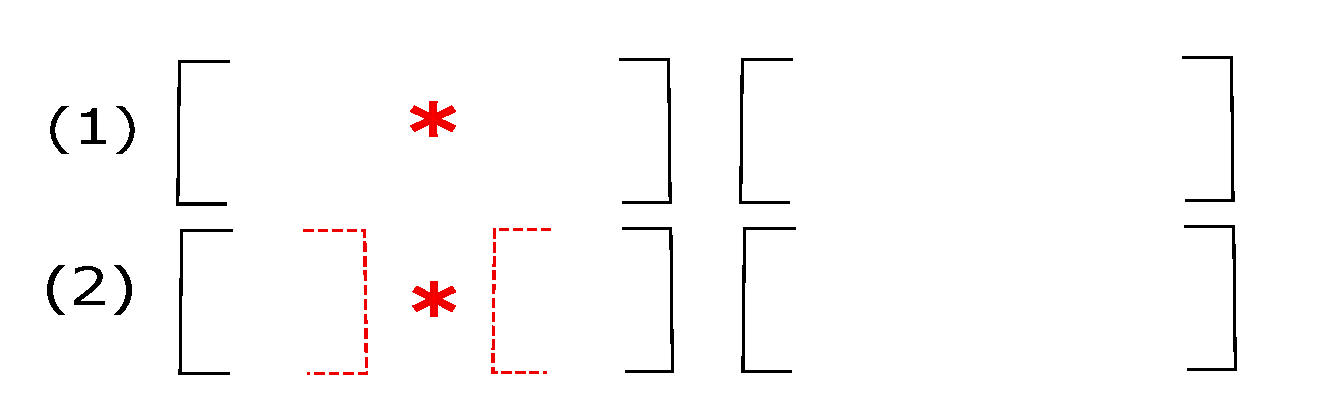
\includegraphics[scale=0.25]{img/attacker_injection_compound.pdf}
	\caption{Example attacker injection when multiple injection points exist in the page. a) a basic injection pattern. b) an attempt to fool the detector.}
	\label{fig:attacker_injection}
	\end{center}
\end{figure}

In Figure~\ref{fig:attacker_injection}a, the brackets indicate a
template. The content in between is an injection point (the star),
where dynamic content is injected into the template. In the case of a
vulnerability, the injected content can expand to any arbitrary
string. The signature separates the injection from the rest by
matching for the start and end points (the \code{endPoints}),
represented by the brackets. This HTML originally has two pairs of
\code{endPoint} patterns.

In Figure~\ref{fig:attacker_injection}b, the attacker knows these are
being used as injection end points and decides to inject a fake ending
point and a fake starting point (the dotted brackets), with some
additional malicious content in between. If just looking for multiple
pairs of end points, the detector cannot tell the difference between
the solid and dotted patterns, and will not get rid of the content
injected in the star. Therefore, we have to use the first starting
point and the last ending point before a starting one (when searching
from the bottom-up) and sanitize everything in between. This might get
rid of a substantial amount of valid HTML, so we defer to the
signature developer's judgment of what behavior the detector should
follow. We expand upon this further in \autoref{case_study}.


\begin{figure}[h]
	\begin{center}
	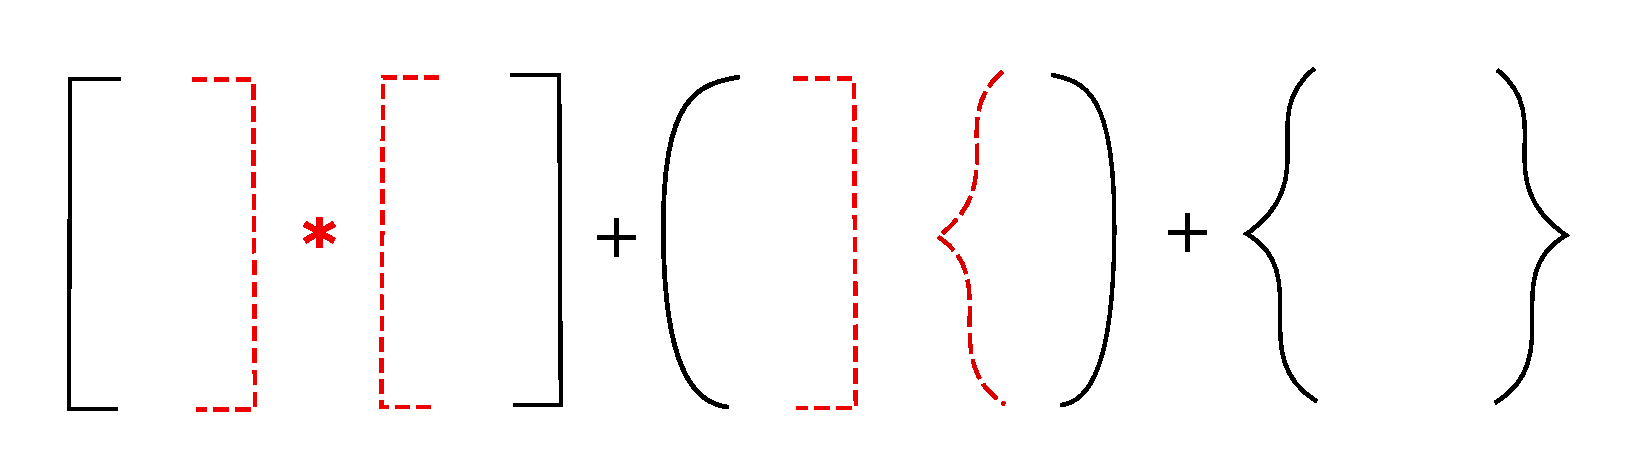
\includegraphics[scale=0.25]{img/attacker_injection_unique.pdf}
	\caption{Example attacker injection when multiple distinct injection points exist in the page.}
	\label{fig:attacker_injection_unique}
	\end{center}
\end{figure}


~\autoref{fig:attacker_injection_unique} illustrates a case when
there are several injection points in one page, but each of them is
distinct. Now, the filter is only looking for one pair of brackets, so
the attacker can't fool the extension into leaving part of the
injection unsanitized. However, they could, for example, inject an
extra ending bracket after the opening parenthesis (or an extra
starting brace). The extension will be tricked into sanitizing
non-malicious content, the black pluses (+). This behavior can be
detected by noting that we know the order in which the
\code{endPoints} should appear, and so if the filter sees a closing
\code{endPoint} before the next expected starting \code{endPoint}, or
similarly, a starting \code{endPoint} before the next expected closing
\code{endPoint}, this attack can be identified. In the diagram, the
order of the solid elements characterizes the possible malformations
in the end points. As with the previous scenario, we have to sanitize
the outermost end points, potentially deleting non-malicious
content. The signature developer specifies the sanitization behavior.

Note that these complex cases do not mean that our approach is not always applicable. The process of writing the signature might become more complicated, but the extension provides a choice for blocking the page entirely if the signature writer believes a given case is too complex for our signature language.

\subsection{Dynamic injections} \label{dynamic_injections}

The top-level documents of web pages fetch additional dynamic content
via \js{fetch} or AJAX APIs. Content fetched in
this way is also vulnerable to \xss, and must be filtered. An example
vulnerability is CVE-2018-7747 (WordPress Caldera Forms, which allows malicious
content retrieved from the plugin's database to be injected in response to a click.

\sys allows XHR requests to be filtered with \js{xhr}-type
signatures. To reduce the number of signatures that need to be
considered when a browser issues a request, we require that signatures
for XHR be nested inside a signature for a top-level document. If a
page's main content matches an existing top-level signature description,
\sys will then enable all nested XHR listeners.

Signatures for dynamic requests are specified in the \js{listenerData}
key, which includes a listener type and method. The idea is extensible
to scripts and other objects loaded separately from the main document
(e.g., images, stylesheets, etc.).

\begin{lstlisting}[breaklines=true,caption={
      An example dynamic request signature. This patches CVE-2018-7747.
    },label={lst:dynamic_signature}]
...
listenerData: [{
  listenerType: 'xhr', listenerMethod: 'POST',
  sanitizer: 'escape', type: 'string',
  listenerUrl: 'wp-admin/admin-ajax.php',
  typeDet: 'single-unique',
  endPoints: ['<p><strong>', '[AltBody]']
}]
\end{lstlisting}


	\section{Implementation}

Our MLCache prototype was built on top of the Linux kernel version 4.14.0-rc7.
In this section, we provide a brief background to the page cache implementation
on Linux and describe how we modified it in order to add the learning model
described in Section~\ref{section:learning}.

\subsection{The Linux Page Cache}

Linux employs a modified version of the traditional LRU strategy called
\emph{two-list LRU}. As the name suggests, two LRU lists are maintained in this
approach: the \emph{active} and \emph{inactive} list. The active list contains
pages that have been accessed more than once in the past, whereas the inactive
list holds the set of pages that have been accessed only once. In other words,
the active list attempts to capture \emph{frequency} and the inactive list
captures \emph{recency}.

The following subsections introduce the main concepts that are relevant to our
work on MLCache. Figure~\ref{fig:lru} describes the two-list approach used in Linux.

\begin{figure}[h]
	\caption{The two-list LRU page cache on Linux. When a page is evicted (last
		page of the inactive list), it is replaced by a shadow page.}
	\label{fig:lru}
\end{figure}

\subsubsection{Dirty Pages}

As mentioned previously, the page cache holds blocks of data stored in the disk
device.  When user space applications perform write operations to certain
blocks of data, the corresponding pages are marked \emph{dirty}. Dirty pages
contain data that has not yet been flushed to the persistence device. In Linux,
dirty pages are not immediately flushed to the disk when the write operation
occurs; instead, the kernel periodically schedules a \emph{ writeback thread}
that scans the LRU lists and writes dirty pages to the disk.

\subsubsection{Cache Eviction}

When pages are read from or written to the disk, new entries are added to the
page cache.  As long as there is enough memory on the system, the number of
pages will keep growing, up to a certain threshold\footnote{Even a special
	webpage was \cite{lamr} created in order to clarify this behavior, which
	probably scares unfamiliar users.}. When the system is under memory pressure,
the kernel will create separate threads that will \emph{shrink} the LRU lists.
In particular, pages at the tail of the inactive LRU list are removed (pages
are always added to the head of an LRU list.) For this reason, Linux also
periodically ensures that the active and inactive lists are balanced: for
example, if too many pages are in the active list, the ones at the tail will be
demoted to the inactive list.

\subsubsection{Page Lookup}

Every page I/O operation on Linux goes through the page cache --- if the an
entry is found (\emph{cache hit}), an expensive call to the disk driver is
saved. Since these page lookups happen very often, they need to take a very
short time to produce a result. Linux 2.6 introduced a new page cache lookup
algorithm using \emph{radix trees} (as opposed to the old, global hash table in
previous kernels.) Each file contains its own radix tree of pages, and lookups
happen by providing only a file offset. Figure~\ref{fig:radix} illustrates the
radix tree approach, as defined in Linux 4.14.0-rc7.

\begin{figure}[h]
	\caption{The Linux page tree. Each file is represented by a (poorly named)
		\texttt{struct address\_space}, and contains a radix tree with pointers to
		locations where pages are kept in memory. When a page is evicted, a shadow
		page is placed in its previous spot. In the example lookup of this figure,
		\texttt{key} resolves to an entry with a shadow page. The corresponding page
		will likely be loaded directly into the \emph{active} LRU list.}
	\label{fig:radix}
\end{figure}

Another important aspect of the Linux implementation of radix trees is that nodes
can be marked with \emph{tags} --- the page cache uses this functionality to
indicate whether pages are dirty, unevictable, or a series of other attributes.
Nodes may also be marked \emph{exceptional}, a feature that is used to detect
shadow pages in the radix tree.

\subsubsection{Shadow Pages} \label{sss:shadow}

Another important optimization employed by the Linux page cache implementation
is the use of \emph{shadow pages}. Whenever a page is evicted, a special entry
--- called shadow page --- is created and replaces the spot previously occupied
by the recently evicted page in the radix tree. When a page lookup occurs and a
shadow page is found at the requested offset, the new page is added to the page
cache and inserted directly into the active LRU list. The use of shadow pages
is a cheap optimization (the shadow page is 8 bytes long, whereas a page is 4 KB
in x86) that can potentially avoid workflows that would cause thrashing.

\subsection{Page Scoring}

MLCache automatically calculates the score for each page based on the algorithm
described in Section~\ref{section:learning}. Specifically, for every page definition
(\texttt{struct page}), MLCache adds two new fields: the current page score, and
the number of times the page was previously evicted. In order for the algorithm
to work, the page scores need to remain accurate at all times.

Fortunately, Linux supports a \emph{tracepoint} API. More precisely, events can be
defined and, once included in a source file, be triggered with certain arguments.
MLCache introduces a new tracepoint, \texttt{mlcache\_event}, which is supposed
to be used whenever a page is requested. The event accepts a series of parameters
including a pointer to the \texttt{struct address\_space} involved, a pointer to the
page itself, the offset requested, and whether it was a hit or a miss. The newly
added event is triggered from within the \texttt{find\_get\_page} function in Linux.

\subsection{The \texttt{mlcache} Driver}

MLCache also introduces a new Linux driver, which coordinates its execution. The
driver's main tasks are:

\begin{description}
	\item[Update page scores] When this driver is loaded, it registers a function to be
	executed whenever the \texttt{mlcache\_event} tracepoint is triggered. This function
	rewards the page being requested and penalizes the other pages in the cache by
	traversing the associated radix tree.
	
	\item[Allow configuration by system operators] While
	MLCache can potentially improve the performance of a large class of applications,
	it is convenient to allow the system operator to selectively choose which applications
	should use MLCache's algorithms. That is done by writing to the \texttt{/proc/mlcache/}
	\texttt{filter}
	file that MLCache creates when it is loaded. Currently, MLCache is able to monitor either
	a list of processes or the process tree under a certain ID. For instance, the command:
	\begin{verbatim}
	echo tree:$$ >/proc/mlcache/filter
	\end{verbatim}
	causes MLCache to monitor every process
	under the running shell.
	
	\item[Read collected information] When monitoring a process, MLCache will create a file
	under the \texttt{/proc/mlcache} directory named after the identifier of the monitored process.
	By reading that file, system operators can analyze statistics about page cache hits/misses.
\end{description}

\subsection{Leveraging Shadow Pages}

As described in \ref{sss:shadow}, Linux uses shadow pages to optimize access to frequently accessed
pages even if they happen to be evicted due to high memory pressure. In our work, we extend the information
contained in the shadow page to include MLCache's scoring data. More specifically, whenever a page
is evicted from the page cache, we include both the current page score, as well as the number of times
the page was previously evicted in the created shadow page. Thus, when a page request finds a shadow
page, it can be brought back to the cache with the score it used to have before evicition. Figure~\ref{fig:shadow}
illustrates how the shadow page is structured when MLCache is enabled.

\begin{figure}[h]
	\caption{The Linux shadow page when MLCache is enabled. Each square
		represents one byte of information.  The shadow page is 8 bytes long and
		contains a series of data --- CPU node identifier, a radix tree entry indicating
		this is an exceptional node, among others. MLCache adds a 4 bytes long page
		score, as well as a 2 bytes long counter, indicating the number of times that
		page was previously evicted.}
	\label{fig:shadow}
\end{figure}

\subsection{Cache Eviction}

The final component of MLCache's implementation is the modified cache eviction policy. Cache eviction
on Linux happens when the amount of memory consumed by the page cache is above a certain threshold.
When pages need to be evicted, kernel threads will be awaken and both the active and inactive
LRU lists may be \emph{shrinked}. The shrinking process happens by evicting the last \texttt{n}
pages in an LRU list (where the value of \texttt{n} is determined at runtime depending on the
system's memory pressure.)

MLCache changes the LRU shrinking process by choosing the pages with the worst score. Unfortunately,
LRU lists are maintained as a linked list of pages, and choosing the pages to evict in LRU is a
constant time operation. Since MLCache needs to determine which pages have the worst score overall,
a linear scan over the LRU list is introduced in this step. Even though better data structures could
be leveraged in order to optimize the eviction process, we see positive results for some workloads
in our benchmarks, despite this unfavorable situation.
	\section{Writing Signatures} \label{signature_writing}

We expect a signature developer to have a solid understanding of the principles behind \ac{XSS}, as well as web applications, HTML, CSS and JavaScript. In this section, we aim to show that minor effort is required from a knowledgeable analyst when writing a signature.


\subsection{Case Study: CVE-2018-10309} \label{case_study}
Going back to our example in Section \ref{motivating_example}, we describe the process for writing a signature using one of our studied CVEs.  

\textbf{Identifying the exploit.} An entry in Exploit Database \cite{studyCVE} describes a persistent \ac{XSS} vulnerability in the WordPress plugin Responsive Cookie Consent for versions 1.7/1.6/1.5. This entry (as most do) comes with a proof of concept (PoC) for the exploit, which describes the Cookie Bar Border Bottom Size parameter as vulnerable. We run a local WordPress installation with this plugin.

\textbf{Establishing the separation between dynamic and static content.} We insert the string \js{"$>$script$>$alert('XSS')$<$/script$>$} in the Cookie Bar Border Bottom Size (rcc\_settings[border-size] in the HTML) input field. This results in an alert box popping up in the page, which has the following HTML:

\begin{lstlisting}
<input id="rcc_settings[border-size]" 
name="rcc-settings[border-size]" 
type="text" value=<@\textcolor{red}{""><script>alert('XSS')</script>}@>
<label class="description"
for="rcc_settings[border-size]">
\end{lstlisting}

In general, the CVE writer is able to find the vulnerable HTML from the server-side code without having to reproduce the exploit. Since we did not write the CVE, we had to do this extra step.

In this case, it is clear that the \textbf{input} element is the injection starting point, and we use the \textbf{label} element as the end point, since it is the element immediately after the \textbf{input}. Identification of correct endpoints is extremely important, and in particular, when a page has multiple injection points, the signature developer must ensure that the chosen elements do not overlap with other innocuous ones. In some cases, the developer might think it best to completely stop the page from loading. While one of our main goals is to maintain the page’s usability, there are cases where large portions of the document would be affected by the sanitization. We believe compromising usability for security is preferable in this case. Furthermore, the developer has to identify if the exploit comes from an external source (such as an Ajax request), as this changes the signature.

\textbf{Collecting other required page information and writing the signature.} The next step is to gather the remaining information to determine whether the signature applies to the page loaded. The full signature for this example was previously shown in Listing \ref{lst:xsnare_signature}. The \textbf{URL} is acquired by noting that this exploit occurs on the plugin's settings page. The \textbf{software} running is WordPress in this case. The settings page's HTML includes a link to a stylesheet with href "http://localhost:8080/wp-content/plugins/responsive-cookie-consent/includes/css/options-page.css?ver=5.2.2", in particular, "wp-content/plugins/plugin-name" is the standard way of identifying that a WordPress page is running a certain plugin. In this case, "responsive-cookie-consent", set as \textbf{softwareDetails}. We apply the signature for all versions less than or equal to 1.7. Since, the exploit only occurs in this specific spot in the HTML, the \textbf{typeDet} is listed as 'single'. 
Since the vulnerable parameter is for border-size, the \textbf{sanitizer} applied is 'regex', further restricting the pattern to only numbers in \textbf{config}. Finally, we list the \textbf{endPoints} as taken from the HTML.

\textbf{Testing the signature}. Finally, we load up our extension and reload the web page. In this example, we expect to not have an alert box pop up, and we manually look at the HTML to verify correct sanitization. In practice, there might be small discrepancies between server-side and client-side representations of the HTML string, leading to bugs in the signature if the developer used the parsed HTML as a reference. If the exploit is not properly sanitized, the developer is able to use the debugging tools provided by the browser to check the incoming network response information seen by the extension's background page and make sure it matches the signature values.

\iffalse
\subsection{Signature writing process}
We describe the process by which a signature is written after a vulnerability has been discovered:
\begin{enumerate}
	\item{
The signature developer crafts a proof of concept exploit for the given CVE. This step is not necessary but it will often help the developer correctly identify the affected areas of the DOM. For our own signatures, we heavily relied on this part because we often did not have the same information as the CVE writer.
Conversely, a knowledgeable analyst will often be able to identify the vulnerable points in the application from the server-side code.}
\item
Using information about where in the HTML the exploit will manifest itself, the developer identifies the start and end points of an injection, and creates regexes to match these. This step is particularly important because this is where the signature might end up covering a bigger part of the DOM than is required, potentially disabling desired functionality, to the detriment of the site user's experience. In particular, when multiple injection points occur in the same page, the developer might find it best to completely stop the page from loading if they think the sanitization would affect the user experience too greatly. While one of our main goals is to maintain the page's usability, there are cases where a large portion of the document would be affected by the sanitization, and we believe compromising usability for security is preferable in this case.

Furthermore, it is at this point where the developer identifies whether the exploit comes in from an external source (such as a response to an Ajax request or an external script) or is embedded in the document's mainframe HTML. This will result in a different signature layout. 
\item
Signatures are loaded for specific pages, and the developer has to specify this information, either via an URL or a regex in the HTML. For example, for a WordPress plugin, the exploit might happen in localhost/plugin-name.php. However, for another exploit, the exploit might occur in a page where the plugin is loaded, which contains the string "wp-content/plugins/plugin-name" in the HTML. Additionally, if the webpage is running pre-defined software, such as WordPress, this has to be specified in the signature as well. Much of this information is already known beforehand, and so this step can be done in conjunction with Step 2.
\item
After the signature has been written, the developer should make sure it was correctly specified. This is most easily done via testing a PoC exploit and verifying the injection has been properly sanitized. For false positives, the developer should make sure that the specified endPoints are uniquely occurring in the HTML (or if not unique, their correct positions have been stated). The browser extension can be used for the purposes of debugging. Some of our most common mistakes when writing signatures were incorrect regexes for the endpoints, and not correctly identifying that the injection occurred as part of an additional network request. These two can be easily fixed by looking through the incoming HTML in the background page's filter. 
\end{enumerate}

\subsection{Case Study: CVE-2018-10309}
Going back to our example in Section 2.4, we describe the full process of writing a signature for one of the CVEs we studied. An entry in Exploit Database \cite{studyCVE} describes a persistent \ac{XSS} vulnerability in the WordPress plugin Responsive Cookie Consent for versions 1.7/1.6/1.5. This particular entry (as most do) comes with a proof of concept for the exploit: 
\begin{enumerate}
\item Access WordPress control panel.
\item Navigate to the Responsive Cookie Consent plugin page.
\item Select one of the input fields. For example, "Cookie Bar Border Bottom Size".
\item Insert the script you wish to inject.
\item Save the plugin settings.
\item Injected script will run in the victim's browser. Depending on which input field you inserted the script, the script may also run everytime you load the Responsive Cookie Consent plugin page.
	
\end{enumerate}

 As described in Section 4.1, in order to test this vulnerability, we find a link to the affected plugin code, and launch a container with a clean installation of WordPress 5.2 with the plugin downloaded. After this, we activate the plugin and proceed to reproduce the proof of concept as described in the Exploit Database entry, inserting the string '">script>alert('XSS')</script>' in the rcc\_settings[border-size] input field, resulting in the following HTML displayed on the page, as well as an alert box popping up in the page:

\begin{lstlisting}
<input id="rcc_settings[border-size]" 
name="rcc-settings[border-size]" 
type="text" value=<@\textcolor{red}{""><script>alert('XSS')</script>}@>
<label class="description"
for="rcc_settings[border-size]">
\end{lstlisting}

In this case, it is clear that the \textbf{input} element is the injection starting point, and we use the \textbf{label} element as the end point, since it is the immediate element after the \textbf{input}. With this information, we are now ready to start writing the corresponding signature, as shown in Listing \ref{lst:xsnare_signature}.

\iffalse
 \lstset{basicstyle=\small}
\begin{lstlisting}
url: 'wp-admin/options-general.php?page=rcc-settings',
software: 'WordPress',
softwareDetails: 'responsive-cookie-consent',
version: '1.7',
type: 'string',
typeDet: 'single-unique',
endPoints: 
['<input id="rcc_settings[border-size]" 
name="rcc_settings[border-size]" type="text"',
'<label class="description" 
for="rcc_settings[border-size]">']
\end{lstlisting}
\fi

The URL is acquired by noting that this exploit occurs on the plugin's settings page, which is in a specific subdomain of the web site. Of course, the software running is WordPress in this case. The settings page's HTML includes a link to a stylesheet with href "http://localhost:8080/wp-content/plugins/responsive-cookie-consent/includes/css/options-page.css?ver=5.2.2", in particular, "wp-content/plugins/plugin-name" is the standard way of identifying that a WordPress page is running a certain plugin. In this case, "responsive-cookie-consent". While the entry only lists versions 1.7, 1.6, and 1.5 as vulnerable, we apply the signature for all versions less than or equal to 1.7.
Since, the exploit only occurs in this specific spot in the HTML, the typeDet is listed as "single-unique". Finally, we list the endPoints as taken from the HTML.

Finally, we load up our extension and reload the web page. In this example, we expect to not have an alert box pop up, and we manually look at the HTML to verify correct sanitization. Note that there's nothing else in between the input and label elements now:

\begin{lstlisting}
<input value="" type="text" 
name="rcc_settings[border-size]" 
id="rcc_settings[border-size]">
<label class="description"
for="rcc_settings[border-size]">
\end{lstlisting}

\fi

	\section{Approach Viability} \label{viability}

To verify the applicability of our detector and signature language, we tested the system by looking at several recent CVEs related to \ac{XSS}. We have three objectives: to verify that our signature language provides the necessary functionality to express an exploit and its patch, to test our detector against existing exploits, and to show that our signature language does not incur a high time overhead when writing a signature.

\subsection{Test methodology} \label{methodology}

Our evaluation focuses on recent CVEs related to WordPress
plugins. While this may seem restrictive, there are several reasons
why we targeted WordPress plugins:
\begin{itemize}
	\item WordPress powers 34.7\% of all websites according to a recent survey  \cite{w3stats}. The same study states that 30.3\% of the Alexa top 1000 sites use WordPress. Thus, we can be confident that our study results will hold true for the average user.
	\item WordPress plugins are very popular among developers (there are currently more than 55,000 plugins \cite{wpplugins}). Due to its user popularity, WordPress is also heavily analyzed by security experts. A search for WordPress CVEs on the Mitre CVE database \cite{cvemitre} gives 2310 results. Plugins, specifically, are an important part of this issue, 52\% of the vulnerabilities reported by WPScan are caused by WordPress plugins \cite{wpscan}.
	\item WordPress plugin code is accessible, so we can easily analyze both the client-side HTML, as well as the server-side code that generated it, which is helpful when writing signatures.
	\item Using one framework, we can install many different plugins for the version we want, reproduce attacks, and investigate the conditions under which they happen, without having to install additional software.
\end{itemize}

We looked at the 100 most recent WordPress \ac{XSS} CVEs, as of October 2018. We have chosen to use a CVE database, CVE Details \cite{cvedetails}, as opposed to other databases that include vulnerabilities or exploits, mainly because of reliability. We have been able to find hundreds of verified attacks on WordPress and its plugins using a CVE database, which also usually contain information on how to reproduce them. This provides the perfect platform to analyze \ac{XSS} attacks and decide whether they can be countered by our approach. 

For each CVE, we set up a Docker container with a clean installation of WordPress 5.2 and installed the vulnerable plugin's version. A few of the CVEs depended on the WordPress version as well, so we used the required WordPress version for those. Of the CVEs we looked at, only one of them occurred in WordPress core. We believe it would be harder to precisely sanitize injection points in WordPress core, as many of the plugins have very particular settings pages where the exploits occur, and the HTML is more identifiable. WordPress core, on the other hand, can be heavily altered by the use of themes and the user's own changes. However, as evidenced by our investigation, the vast majority of exploits occur in plugins.
 
 We then reproduced the exploit as described by the CVE. Finally, we analyzed the vulnerable page and wrote a signature to patch the exploit.

\subsection{Results}

\begin{table}[h!]
	\begin{center}
		\begin{tabular}{|c c|} 
			\hline
			Plugin & Installations\\ [1ex] 
			\hline
			WooCommerce  & 5+ million  \\  
			Duplicator & 1+ million \\  
			Loginizer & 900,000+ \\  
			WP Statistics & 500,000+ \\  
			Caldera Forms & 200,000+ \\   
			\hline
		\end{tabular}
		\caption{Most popular studied WordPress plugins}
		\label{table:1}
	\end{center}
\end{table}

Of the initial 100 CVEs, we were able to analyze 76 across 40 affected pages. We dropped 24 CVEs due to reproducibility issues: some of the descriptions did not include a PoC, making it difficult for us to reproduce; or, the plugin code was no longer available. In some cases, it had been removed from the WordPress repository due to "security issues", which emphasizes the importance of being able to defend against these attacks. This is not to say, however, that our detector would not work for such a CVE, as the author would have a better idea of how the exploit manifests itself, and would be in a better position to write a signature. The plugins we studied averaged 489,927 installations; \autoref{table:1} shows the number of installations for the 5 most popular studied plugins. For the vulnerabilities, 27 (35.5\%) could be exploited by an unauthenticated user; 56 (73.7\%) targeted a high-privilege user as the victim, 7 (9.2\%) had a low-privilege user as the victim, the rest affected users of all types.

Many of the studied CVEs included attacks for which there are known and widely deployed defenses. For example, many were cases of Reflected \ac{XSS}, where the URL revealed the existence of an attack, e.g:


$http://[path to WordPress]/wp-admin/admin.php?page=wps\_pages\_page\&page-uri=<script>alert("\ac{XSS}")</script>$

While Chrome's built-in \ac{XSS} auditor blocked this request, Firefox did not, and so we still wrote signatures for such attacks. In practice, we found several cases where even XSS auditor did not block the reflected XSS. We wrote 59 WordPress signatures in total, which got rid of the PoC exploit when sanitized with one of our three methods. Note that while PoCs are often the most simple form of an attack, our sanitization methods, and in particular DOMPurify, can get rid of complex injections as well. We were able to include several CVEs in some of them because they occurred in the same page and affected the same plugin. Overall, these signatures represent 71 (93.4\%) signed CVEs. The 5 we were not able to sign were due to lack of identifiers in the HTML, which would result in potentially large chunks of the document being replaced. For cases like these, the signature developer can weigh the trade-offs and decide whether the added cost is worth it.

After manual testing, the majority of the 71 signatures maintained the same layout and core functionality of the webpage. However, 12 signatures caused some elements to be rearranged, modifying the page's visual aspect. One caused a small part of the page to become unusable, due to the sanitization method used (a table showing user information was now rendered as blank). Most of the responsibility of maintaining functionality is left to the signature developer, being as precise as possible is key.

While our goal is to retain as much information of the page as possible after sanitization, we believe that even if a part of the page is now useless, this does not impact the user's experience as much, since most of these exploits occur in small sections of the HTML. A thorough study with regards to usability is out of scope for this work, but we provide some insight into false positives and false negatives in later sections, which is related to this issue.

\subsection{Generalizability} \label{generalizability}

To test the generalizability of our approach to other frameworks, we
analysed 5 additional CVEs, 2 related to Joomla!, 2 for LimeSurvey,
and 1 for Bolt CMS.  We chose Joomla! because it is another
popular \ac{CMS}. Unfortunately, we only found 2 CVEs
that we were able to reproduce, as the software for its extensions is
often not available. For fairness, we looked for the most recent CVEs
we could reproduce listed in the Exploit Database~\cite{exploitdb}, since
these have recorded \acp{PoC}. We carried out the same
procedure as with the WordPress CVEs, and were able to patch all of
the 5 exploits. This brought our CVE coverage rate up to 94.2\%.

\subsection{Signature writing times} \label{signature_times}

Figure ~\ref{fig:signature_times} shows a histogram of the time taken to write each of our signatures: this includes the time taken to check the HTML injection points, write the signature and debug it. We do not include the time taken to discover and carry out an exploit, as this is part of the CVE writing process. The median time is 3.89 minutes, and the standard deviation is 4.18 minutes. 72\% of signatures took less than 5 minutes to write. We believe this to be a reasonable amount of time for the security granted by our extension.

The signature which took the longest to write (25 minutes) corresponded to an exploit which had several injection points in the HTML, 12 exactly. Additionally, testing this signature proved more difficult than others, as some of the injections were a result of a script inserting elements in the DOM after the page had loaded. This caused the initial HTML to look innocuous, but with exploits still occurring after sanitization. As this script was part of the initial request, we eventually got to the root of the problem. We believe a more experienced exploit analyst might be able to detect this kind of behaviour more easily. Furthermore, having so many injection points in the HTML is cause for great complexity, and the writer can decide to block the page entirely, which would bring down the time taken.

Similarly, the second longest time taken (18 minutes) corresponded to an exploit which had 7 injection points, but each of these belonged to a part of the HTML with very generic element identifiers. Our language provides a means to overcome this, by being able to specify the element's "position": for example, if there are three <h3 class="title"> elements, in the HTML, and only one of them is an injection starting point, the writer can specify that the third one needs to be sanitized. The same happens for the ending points. As there were 7 of these such points, debugging took longer than for most of the other signatures. Again, this is a very complex case, and can be more prone to user error than other signatures, the writer might instead decide to block the page entirely.

Note that we have some signatures which cover several CVEs, as sometimes one page can have multiple CVEs associated with it. In particular, we had 6 of these, which had a median write time of 6.54 minutes. This means that the time per CVE is lower than the overall median of 3.89. Another source of increase timing is the more complicated case of listener type signatures, like ones for exploits caused by an XHR. We had 4 of these signatures, with a median write time of 9.86. As only a small number of these were present, we expect the time taken to write an average signature to be lower than the calculated total median.

\begin{figure}[h]
	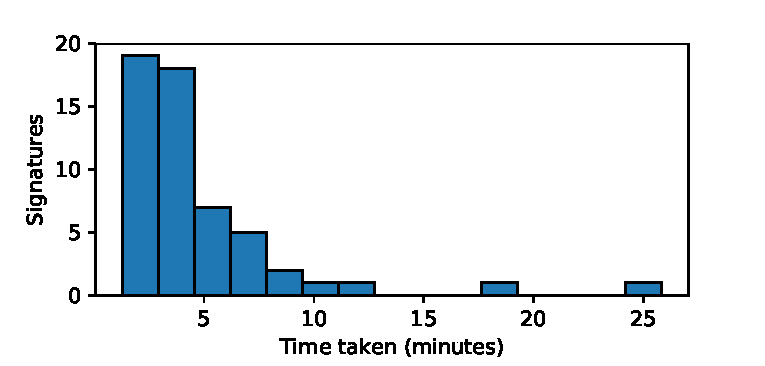
\includegraphics[scale=0.5]{results/signature_times_small.pdf}
	\caption{Histogram of time taken to write signatures.}
	\label{fig:signature_times}
\end{figure}



	\section{Performance Evaluation} \label{performance}
The extension's performance goals are to provide our security guarantees without being a detriment to the end user's browsing experience. To this end, we take several timestamps throughout our code's execution. These were recorded using the Performance Web API. Note that while this API normally reports values as doubles, due to recent security threats, such as Spectre \cite{DBLP:journals/corr/abs-1801-01203}, several browser developers have implemented countermeasures by reducing the precision of the DOMHighResTimeStamp resolution \cite{reducetimeprecision,resolutionconsiderations}. In particular, Firefox reports these values as integer milliseconds. For our tests, we re-enabled higher precision values.

While our extension's functionality only applies at the network level, there is potential slowdown at the DOM processing level due to the optimization techniques the browser applies throughout several levels of the web page load pipeline. Figure ~\ref{fig:navigationtiming} shows the different timestamps provided by the Navigation Timing API \cite{navigationtiming}, as well as a high-level description of the browser processing model. Since our filter listens on the onBeforeRequest event, none of the previous steps before Request are affected. In this section, we refer to the difference in time between responseEnd and requestStart as the "network filter time".

\begin{figure*}[h]
 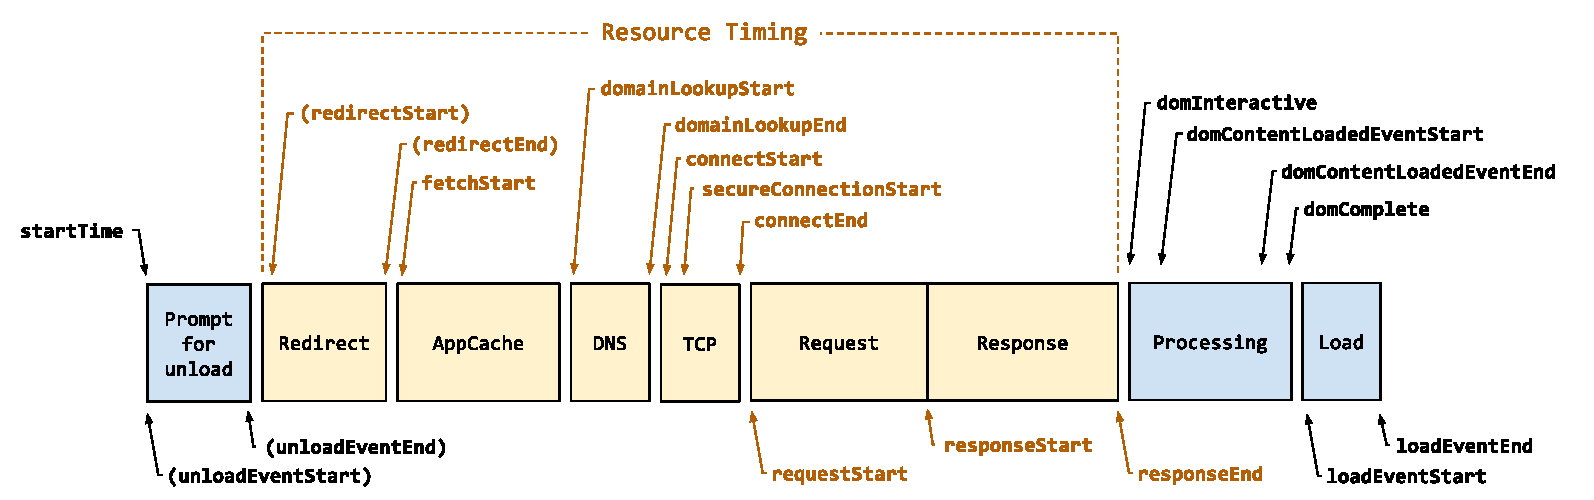
\includegraphics[scale=0.65]{img/timestamp-diagram.pdf}
 \caption{The Navigation Timing API's timestamps\protect\footnotemark}
 \label{fig:navigationtiming}
 \end{figure*}


\subsection{Top websites load times} \label{top_sites}
We first report our extension's impact on top website load times, representing the expected behaviour of an user's average web browsing experience. For these tests, we first took the top 500 websites as reported by Moz.com \cite{top500}. For each website, we loaded it 25 times (with a 25 second timeout) and recorded the following values: requestStart, responseStart, responseEnd, domContentLoadedEventEnd, domComplete, duration, and decodedBodySize. From the initial 500, we only report values for 441 of them. The other 59 had consistent issues with timeouts, insecure certificates, and network errors. For our setup, we used a headless version of Firefox 6.90, and Selenium WebDriver for NodeJS, with GeckoDriver. All experiments were run on one machine with an Intel Xeon CPU E5-2407 2.40GHz processor, 32 GB DRAM, and our university's 1GiB connection. We ran four test suites:
\begin{itemize}
	\item No extension cold cache: Firefox is loaded without the extension installed and the web driver is re-instantiated for every page load.
	\item Extension cold cache: Firefox is loaded with the extension installed and the web driver is re-instantiated for every page load.
	\item No extension warm cache: Firefox is loaded without the extension installed and the same web driver is used for the page's 25 loads.
	\item Extension warm cache: Firefox is loaded with the extension installed and the same web driver is used for the page's 25 loads.
\end{itemize}

For each set of tests, we reduced the recorded values to two comparisons: network filter (responseEnd - requestStart), and page ready (domComplete - responseStart). The first analyzes the time spent by the network filter, while the second determines the time spent until the whole document has loaded. We calculate the medians for each website for each of these measures as well as the decodedByteSize.

\begin{figure}[h]
	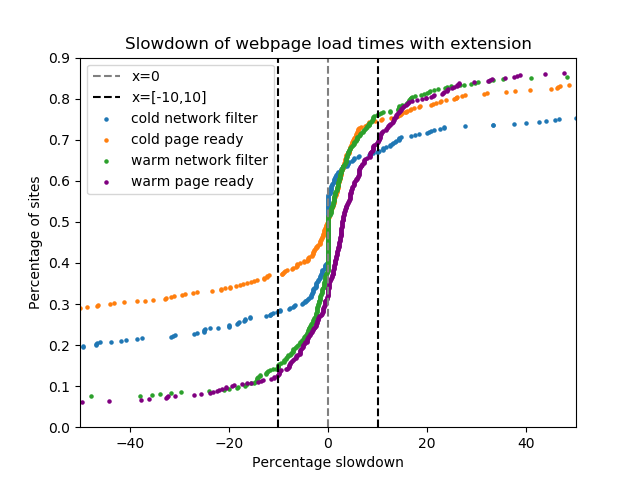
\includegraphics[scale=0.5]{results/extension_slowdown_overall.png}
	\caption{Cumulative distribution of relative percentage slowdown with extension installed for top sites.}
	\label{fig:overall_slowdown}
\end{figure}

We compare the load times with and without the extension running by calculating the relative slowdown with the extension installed according to the following formula: 

\begin{equation*}
100*\frac{\tilde{x}_{with}-\tilde{x}_{without}}{\tilde{x}_{without}}
\end{equation*}
\\
where $\tilde{x}$ is the median with/without the extension running.

Figure ~\ref{fig:overall_slowdown} shows the computed results. We have zoomed in on the $[-50\%,50\%]$ range, as this is where the grand majority of values lie. The graph shows a slowdown of less than 10\% for 72.6\% of sites, and less than 50\% for 82\% of sites when the extension is running. Note that these values are recorded as percentages, and while some are as high as 50\%, the absolute values are in 77\% of cases less than a second. This overhead should not alter the user's experience significantly. The slowdown increases by at most 5\% when we take caching into account. We expect this to be the case because the network filter probably causes the browser to use less caching, especially for the DOM component, as it might have to process it from scratch every time.

\begin{figure}[h]
	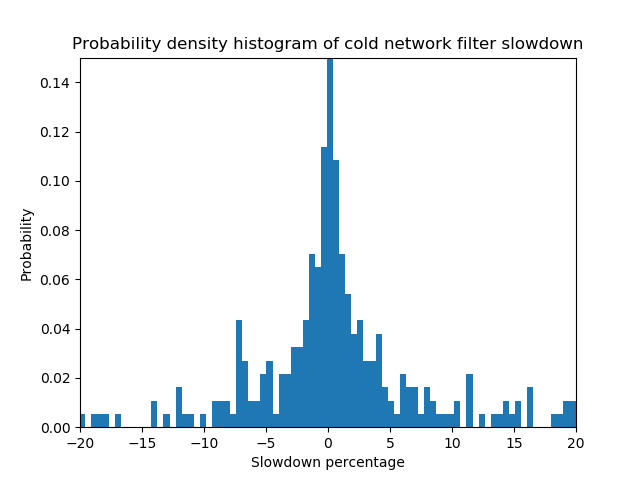
\includegraphics[scale=0.5]{results/density_histogram_filter_slowdown.png}
	\caption{Density histogram of network filter slowdown for top sites.}
	\label{fig:histogram_slowdown}
\end{figure}


Figure ~\ref{fig:histogram_slowdown} shows a closer look at the distribution for the cold network filter slowdown on the top sites (same values as in \autoref{fig:overall_slowdown}). We filtered out any values above |100|\%, as these were mostly due to timeouts and other network delays or errors. For this component, 87.6\% of the slowdown values are less than 10\%.

\begin{figure}[h]
	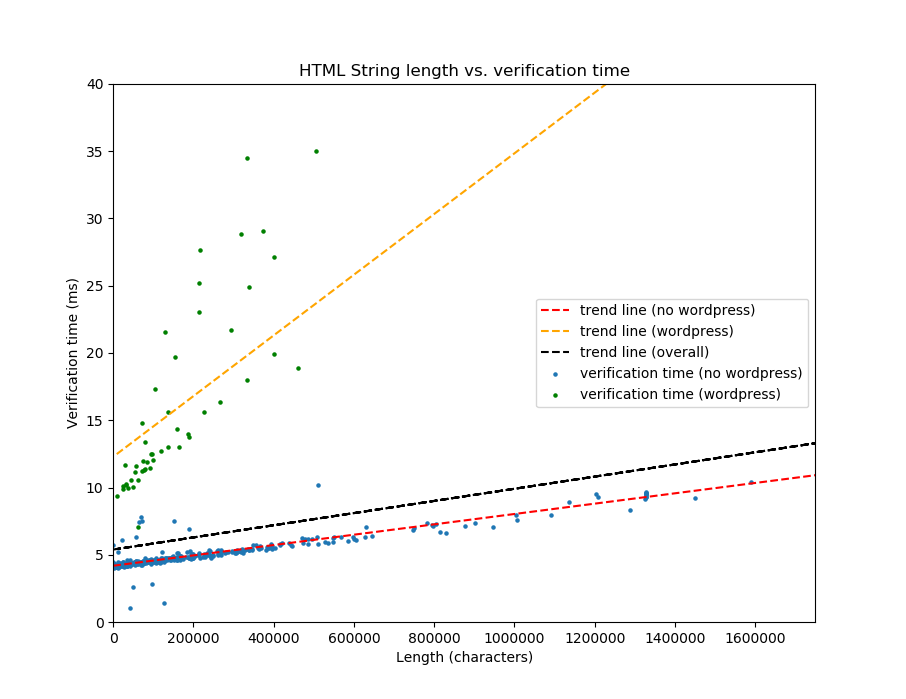
\includegraphics[scale=0.37]{results/string_length_vs_verification_time.png}
	\caption{Scatter plot of network filter time as a function of decoded byte size for top sites.}
	\label{fig:verification_time_string_length}
\end{figure}

 Figure ~\ref{fig:verification_time_string_length} shows the time spent by the call to our string verification function in the network filter as a function of the length of the string to be verified. We loaded the same websites 25 times each and calculated the median times and lengths.  The blue dots are the pages for which the WordPress probes tested negative, and the green dots are the pages for which the probes tested positive: 55 in total (our implementation currently only has probes for WordPress). We applied least squares regression to calculate the shown trend lines. The Spearman's rank correlation values for no WordPress, WordPress, and overall are 0.91, 0.91, and 0.72 respectively, demonstrating positive correlation. Since both our probes and signatures use regex matching, we expect both trend lines to be linear, as seen in the graph. Recall that once a probe for a certain software passes, we perform a linear scan over the signatures for that specific software and check whether it applies to the given HTML string or not. Thus, we expect the slope of the line to be higher when the WordPress probe passes. Since only around 25\% of sites use WordPress on average \cite{w3techs}, we expect the impact of our network filter to be closer to the non-WordPress values, as corroborated by our overall trend line.

\footnotetext{This image was taken from the w3 spec: \url{https://www.w3.org/TR/navigation-timing-2/}}

Additionally, for each website we recorded the number of loaded signatures (i.e., signatures whose endpoints were found in the HTML). We report a 0\% false positive rate for loaded signatures. Thus, we can infer with confidence that the rate of false positives for loaded signatures during an average user's web browsing is similarly low. This rate could possibly go up as the number of signatures and covered frameworks increases. While we can not be sure that any of the sites is free of vulnerabilities described in our current signatures, this is very unlikely, as many of these websites are not running WordPress to begin with, and being some of the most popular, they would likely be updated relatively quickly if any vulnerability is found; thus, the rate of false negatives is likely extremely low as well.

\subsection{Wordpress websites load times} \label{wordpress_sites}

We ran similar experiments as in Section 6.1, but with the WordPress sites described in Section 4.1. Thus, all of these have either one or multiple injection points in their HTML, and the network filter will spend an additional amount of time sanitizing these as defined by the signatures. Note that the data set is smaller here, and some of the trends might be harder to infer. 

As before, Figure ~\ref{fig:wordpress_slowdown} shows the results for slowdown with the extension running. Recall that the only difference between a page which passes the WordPress probe and one that matches a signature is that the latter has to replace a portion of the original string by its sanitized version. This procedure is usually very fast, and can be faster depending on the method defined by the signature. Since even some of the top 500 sites ran WordPress, we expect a minimal difference between the two data sets. In this case we see a slowdown of less than 10\% for 88.75\% of sites, and less than 40\% for 98.75\% of them. The warm curves suffer from a smaller slowdown than the cold ones. We believe this to be the case because of the very small load times when caching is taken into account due to these pages being locally hosted, thus even minor changes in load times result in higher absolute slowdowns.

\begin{figure}[h]
	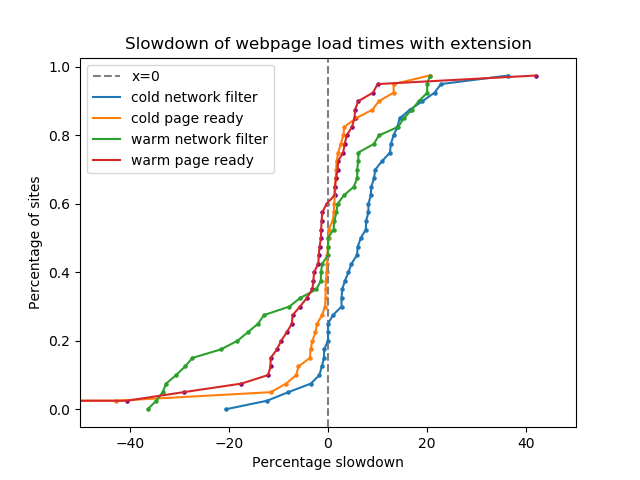
\includegraphics[scale=0.5]{results/extension_slowdown_wordpress.png}
	\caption{Cumulative distribution of relative percentage slowdown with extension installed for WordPress sites.}
	\label{fig:wordpress_slowdown}
\end{figure}

Figure ~\ref{fig:histogram_slowdown_wordpress} shows the probability density of the cold network filter slowdown. In this case, we see that the distribution is skewed more towards a higher slowdown. As it is harder to discern the trend for this data set than its top site counterpart, we have also plotted the normal distribution of the data between 3 standard deviations. 65\% of values are less than 10\%.

\begin{figure}[h]
	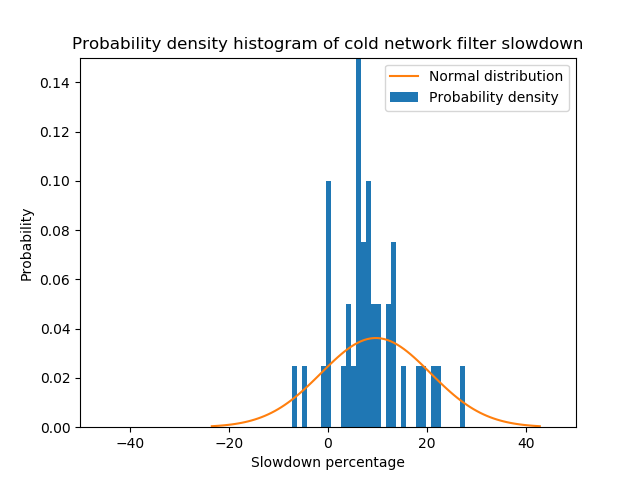
\includegraphics[scale=0.5]{results/density_histogram_filter_slowdown_wordpress.png}
	\caption{Density histogram of network filter slowdown for top sites.}
	\label{fig:histogram_slowdown_wordpress}
\end{figure}

Finally, we report the string verification time as a function of its length, for the WordPress sites, shown in Figure ~\ref{fig:verification_time_string_length_wordpress}. The Spearman's rank correlation for this set of data is 0.630. 

\begin{figure}[h]
	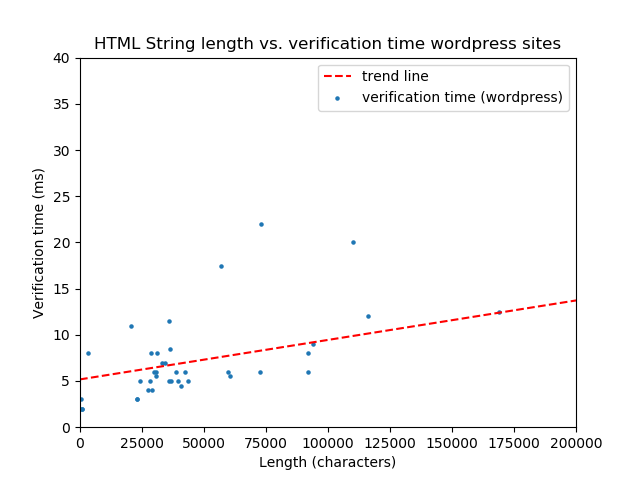
\includegraphics[scale=0.5]{results/string_length_vs_verification_time_wordpress.png}
	\caption{Scatter plot of network filter time as a function of decoded byte size for WordPress sites.}
	\label{fig:verification_time_string_length_wordpress}
\end{figure}
	\section{Limitations and Future Work}

\textbf{Generalizability and scope of study.} As discussed in \autoref{methodology}, while many websites share similar structures to the ones we covered, our study only considered 4 other sites apart from those running on WordPress, and we only considered sites using a CMS. Not all websites might be identified as easily. Furthermore, we only studied 81 CVEs. %% , 24 of which had to be discarded in our analysis
In the future we intend to study a more diverse set of CVEs and go beyond CMS-based sites.
% in the future to have a better representation of WordPress websites, plugins, and the web as a whole.

\textbf{False positives and false negatives.} It is extremely hard to get completely rid of FPs. If the sanitization targets JavaScript code, for example, a FP will likely be triggered. Furthermore, since we rely on handwritten signatures, vulnerable sites for which no signature has been written will be subject to FNs. In the future, we intend to study the rate of FPs and FNs in our approach and compare it to previous work.

%% Faulty sanitization could be reduced by implementing our sanitization methods as a lexer instead of the declarative version we currently have: The signature developer would ideally provide the allowed behaviour in a given injection point, and the detector would check the injection content against the specified behaviour, providing a proof of whether the content could have been generated by following the rules. This would make sanitization more accurate.

%\textbf{Usability.} A main aspect of our work is its increased potential for usability and adoption from both a user's perspective that installs the extension to defend themselves against \ac{XSS}, and a signature developer who has to write the database descriptions according to a known CVE. Future work could focus on usability studies related to both of these aspects.

\textbf{Protection against CSRF.} We believe that we can adapt our work to defend against \ac{CSRF} exploits, as well. Using a similar signature language as the one for \ac{XSS}, a signature developer could specify pages with potential vulnerabilities to only allow network requests that cannot exploit such vulnerabilities.

%% While our work has only focused on \ac{XSS}, we believe we can easily adapt our network filter to defend against \ac{CSRF} exploits as well. Using a similar signature language as the one for \ac{XSS}, a signature developer could specify pages with potential vulnerabilities to only allow network requests that can not exploit such vulnerabilities. In some scenarios, it might be useful to track DOM events, e.g., user clicks to protect against click-jacking attacks. This kind of information is not available to the network; however, the extension could install a script on the page to monitor these actions.

\textbf{Filtering network data.} Our filter's design depends
on Firefox's implementation of the WebRequest API.
Firefox's filterResponseData method allows the extension to modify an incoming
HTTP request\footnote{https://developer.mozilla.org/en-US/docs/Mozilla/Add-ons/WebExtensions/API/webRequest/filterResponseData}.
This feature has been requested in other browsers like
Chrome, but it has not been implemented. This design limits our deployability to Firefox users.

%% As of September 2019, CVE Details had 14894 \ac{XSS} vulnerabilities in its database \cite{vulnbytype}. This means that our current signatures only cover 0.5\% of all existing \ac{XSS} vulnerabilities. More efficient approaches at searching and filtering, as well as for the data structures used in the signature database could be applied to maintain a low performance overhead. The task of signature filtering, for example, is embarrassingly parallel in the number of signatures.

\textbf{Design considerations}. Currently, each browser user has to install our extension. However, the same functionality could be offloaded to a single processing unit similar to a proxy, which can handle the filtering for all machines in a network. This deployment model might be more appropriate in certain environments, such as in enterprises.

%% While any user could alter their local signature database, most will not have the technical expertise to do so. However, a trusted community of users could flag websites as being potentially malicious as part of a separate database, saving time for others.

%% We continue working on the system to make it more robust, both in terms of being able to defend against a myriad of attacks, as well as providing ease of development for signatures.

	\section{Related Work}
We classify existing work into multiple categories: client-side, server-side, browser built-in, and hybrid: a combination of these.

\noindent \textbf{Server-side techniques.}
In addition to existing parameter sanitization techniques,
taint-tracking has been proposed as a means to consolidate
sanitization of vulnerable parameters~\cite{Xu:2006:TPE:1267336.1267345,DBLP:conf/sec/Nguyen-TuongGGSE05,Pietraszek:2005:DAI:2146257.2146267,Bisht:2008:XPD:1428322.1428325}. These
techniques are complementary to ours, and provide an additional line
of defence against \ac{XSS}. However, many of them rely on the
client-side rendering to maintain the server-side properties, which
will not always be the case.

\noindent \textbf{Client-side techniques.}
DOMPurify~\cite{10.1007/978-3-319-66399-9_7} presents a robust
\ac{XSS} client-side filter. The authors
argue that the DOM is the ideal place for sanitization to occur. While
we agree with this view, their work relies on application developers
to adopt their filter and modify their code to use it. Thus, we have partly automated this step by including it as our default sanitization function.

Jim et al.~\cite{Jim:2007:DSI:1242572.1242654} present a method to
defend against injection attacks through Browser-Enforced Embedded
Policies. This approach is similar to ours, as the policies specify
prohibited script execution points. However, this again relies on application developers knowing where their code might be vulnerable. Furthermore, browser modifications are required to benefit from it. Similarly, Hallaraker and Vigna~\cite{Hallaraker:2005:DMJ:1078029.1078861} use a
policy language to detect malicious code on the client-side. Like \sys, they make use of signatures to protect against known types of
exploits. However, unlike our approach, their signatures are not
application-specific, and there is no model for signature
maintenance. Furthermore, there is no evaluation on the efficacy of
their signatures.

Snyder et al.~\cite{Snyder:2017:MWD:3133956.3133966} report a study in which
they disable several JavaScript APIs and test the number of websites
that are do not work without the full functionality of the APIs. This approach increases security due to vulnerabilities present in several
JavaScript APIs, however, we believe disabling API functionality
should only be used as a last resort.

\noindent \textbf{Browser built-in defences.}  Browsers are equipped
with several built-in defences. We previously described XSS
Auditor in \autoref{introduction}, the other two important ones are Content
Security Policy and the Same-origin policy.

\ac{CSP}~\cite{CSP} has been widely adopted and
in many cases provides developers with a reliable way to protect
against \ac{XSS} and \ac{CSRF} attacks. However, \ac{CSP} requires the developer to know which scripts
might be malicious.

Same-origin policy~\cite{SOP} is another useful security mechanism for
protection against \ac{XSS} and \ac{CSRF}. This policy restricts how a
document or script loaded from one origin can interact with a resource
from another origin. However, if the attack is injected in the same
website the attacker intends to compromise, this will not defend
against it. As with other approaches these browser policies are complementary to \sys.

\noindent \textbf{Client and server hybrids.}
XSS-Dec~\cite{Sundareswaran:2012:XHS:2352970.2352994} uses a proxy which keeps track of an encrypted version of the server's source files, and applies this information to derive exploits in a page visited by the user. This approach is similar to ours, since we assume previous
knowledge of the clean HTML document. Furthermore, they user anomaly-based and signature-based detection to prevent attacks. However, there is no mention of signature maintenance. In a way, our system offloads all this functionality to the client-side, without the need of any server-side information.


	\section{Conclusion}

Users cannot depend on administrators to patch vulnerable server-side
software or for developers to adopt best practices to mitigate XSS
vulnerabilities. Instead, users should protect themselves with a
client-side solution. In this paper we described the design,
implementation, and evaluation of one such client-side approach in
\sys.
%
\sys prevents \ac{XSS} exploits by using a database of exploit
signatures and by using a novel mechanism to detect XSS exploits in a
browser extension.
%
We evaluated our approach through a study of 104 CVEs in which we
showed that our tool defends against 93.75\% of the exploits.

%% We have presented \sys, a fully client-side protection mechanism
%% against XSS.
%% \sys has many benefits over existing
%% systems, as well as being complementary to many of them. 
%% The \sys firewall
%% architecture allows users to protect themselves in the face
%% of an ever-increasing number of potential attacks and attack vectors,
%% with little additional effort required for a knowledgeable security
%% analyst when taking into consideration the existing vulnerability
%% detection work flow.



%%  we conducted showed that the provided API for
%% sanitization and injection point detection is effective, as 93.75\% of
%% these vulnerabilities could be defended with \sys. Our \sys prototype
%% meets the required performance goals to not be detrimental to a user's
%% web experience, as web page load times increase by less than 10\% on
%% 72.6\% of sites.

	\appendix

%%%%%%%%%%%%%%%%%%%%%%%%%%%%%%%%%%%%%%%%%%%%%%%%%%%%%%%%%%%%%%%%%%%%%%%%
\section{Performance evaluation} \label{appendix:perf-eval}
%%%%%%%%%%%%%%%%%%%%%%%%%%%%%%%%%%%%%%%%%%%%%%%%%%%%%%%%%%%%%%%%%%%%%%%%

In this section we report additional performance measurements for \sys
to gauge how well it meets its goals.

\textbf{Methodology.} We recorded timestamps while our code is
executing using the Performance Web API\footnote{Note that while this
  API normally reports values as doubles, due to recent security
  threats, such as Spectre~\cite{DBLP:journals/corr/abs-1801-01203},
  several browser developers have implemented countermeasures by
  reducing the precision of the DOMHighResTimeStamp
  resolution~\cite{reducetimeprecision,resolutionconsiderations}. In
  particular, Firefox reports these values as integer
  milliseconds. For our tests, we re-enabled higher precision values.}

While our extension's functionality only applies at the network level,
there is potential slowdown at the DOM processing level due to the
optimization techniques the browser applies throughout several levels
of the web page load pipeline. \autoref{fig:navigationtiming} shows
the different timestamps provided by the Navigation Timing
API~\cite{navigationtiming}, as well as a high-level description of
the browser processing model. Since our filter listens on the
onBeforeRequest event, none of the previous steps before Request are
affected. In this section, we refer to the difference in time between
responseEnd and requestStart as the "network filter time".

\begin{figure}[h]
	\begin{center}
 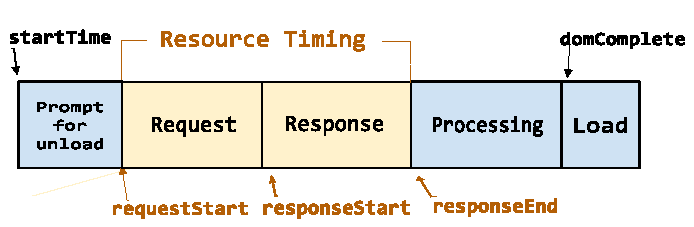
\includegraphics[scale=0.65]{img/timestamp-diagram-edited.pdf}
 \end{center}
 \caption{The Navigation Timing API's timestamps\protect\footnotemark}
 \label{fig:navigationtiming}
 \end{figure}

\footnotetext{This image was taken from the w3 spec: \url{https://www.w3.org/TR/navigation-timing-2/}}


\subsection{Top websites load times; continued} \label{top_sites}

\iffalse
\begin{figure}[h]
	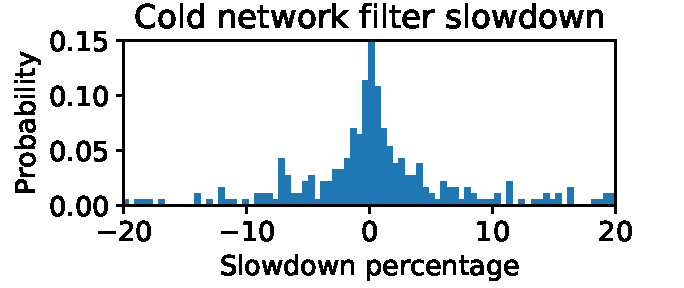
\includegraphics[scale=0.5]{results/density_histogram_filter_slowdown_small.pdf}
	\caption{Density histogram of network filter slowdown for top sites.}
	\label{fig:histogram_slowdown}
\end{figure}


Figure ~\ref{fig:histogram_slowdown} shows a closer look at the distribution for the cold network filter slowdown on the top sites (same values as in \autoref{fig:overall_slowdown}). For this component, 87.6\% of the slowdown values are less than 10\%.
\fi

\begin{figure}[h]
	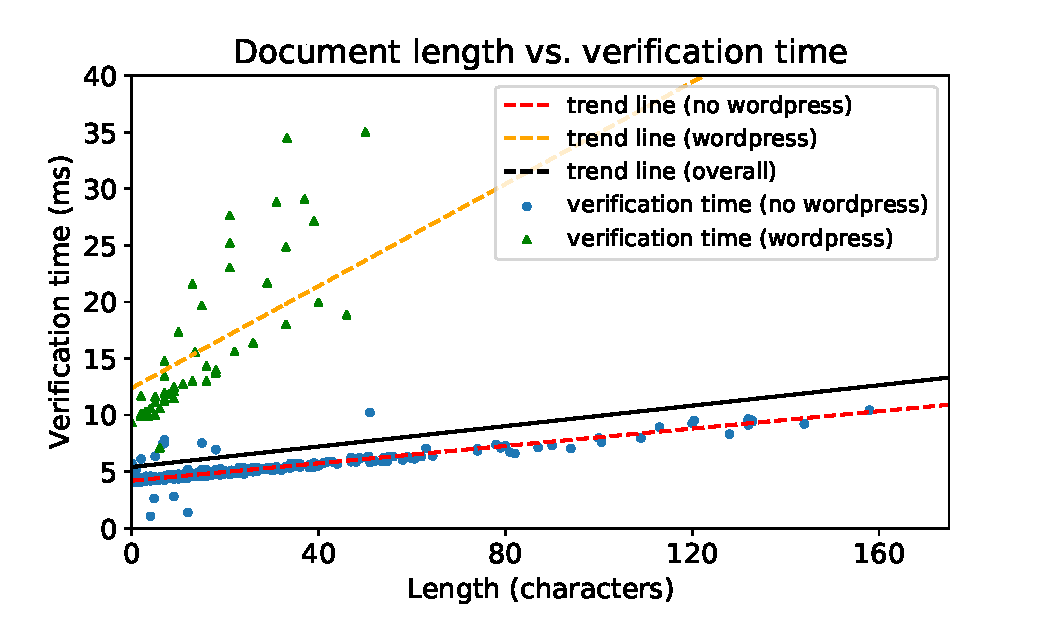
\includegraphics[scale=0.5]{results/string_length_vs_verification_time_small.pdf}
	\caption{Scatter plot of network filter time as a function of character length for top sites.}
	\label{fig:verification_time_string_length}
\end{figure}

 \autoref{fig:verification_time_string_length} shows the time spent by the call to our string verification function in the network filter as a function of the length of the string to be verified. The blue dots are the pages for which our framework probes tested negative, and the green triangles are the pages for which the probes tested positive: 55 in total. We applied least squares regression to calculate the shown trend lines. The Spearman's rank \footnote{The Spearman's correlation coefficient measures the strength and direction of association between two ranked variables: https://statistics.laerd.com/statistical-guides/spearmans-rank-order-correlation-statistical-guide.php} correlation values for no probe, probe, and overall are 0.91, 0.91, and 0.72 respectively, demonstrating positive correlation. Since both our probes and signatures use regex matching, we expect both trend lines to be linear, as seen in the graph. Recall that once a probe for a certain software passes, we perform a linear scan over the signatures for that specific software and check whether it applies to the given HTML string or not. Thus, we expect the slope of the line to be higher when a probe passes. Around 37.4\% of all web sites use frameworks covered by our probes~\cite{w3stats}, thus, we expect the impact of our network filter to be closer to the non-probe values, as corroborated by our overall trend line.
 

\textbf{False positives on the Web.} Additionally, for each website, we recorded the number of loaded signatures. We report a 0\% FP rate for loaded signatures. Thus, we can infer with confidence that the rate of false positives for loaded signatures during an average user's web browsing is similarly low. This rate could possibly go up as the number of signatures and covered frameworks increases. It is likely that these websites are free of vulnerabilities covered by our signatures, as many of these websites are not running WordPress to begin with, and being the most popular, they would likely be updated quickly if a vulnerability is found; thus, the rate of false negatives is likely extremely low as well.

\subsection{WordPress websites load times} \label{wordpress_sites}

We ran similar experiments as in Section 6.1, but with the WordPress sites described in Section 4.1. Thus, all of these have either one or multiple injection points in their HTML, and the network filter will spend an additional amount of time sanitizing these as defined by the signatures. Note that the data set is smaller here, and some of the trends might be harder to infer.

\autoref{fig:WordPress_slowdown} shows the results for slowdown with the extension running for these sites. Recall that the only difference between a page which passes the WordPress probe and one that matches a signature is that the latter has to replace a portion of the original string by its sanitized version. In this case we see a slowdown of less than 10\% for 60\% of sites, and less than 40\% for 96.25\% of them. The warm network filter curve suffers from a particularly high slowdown. We believe this to be the case because the locally hosted pages decrease the network component time, causing any overhead to be seen as relatively high. However, as 48\% of the original values were below 60ms, conclude a small impact on user experience as well.

\begin{figure}[h]
	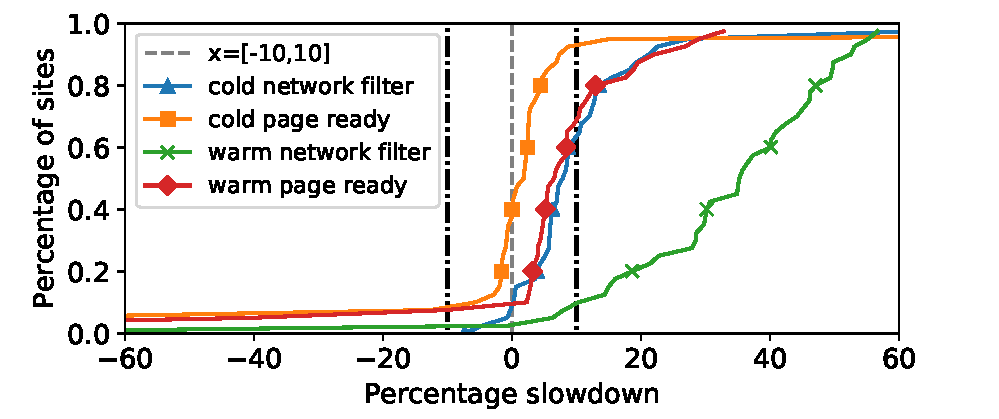
\includegraphics[scale=0.5]{results/extension_slowdown_wordpress_small.pdf}
	\caption{Cumulative distribution of relative percentage slowdown with extension installed for WordPress sites.}
	\label{fig:WordPress_slowdown}
\end{figure}

\iffalse
\autoref{fig:histogram_slowdown_wordpress} shows the probability density of the cold network filter slowdown. In this case, we see that the distribution is skewed more towards a higher slowdown. As it is harder to discern the trend for this data set than its top site counterpart, we have also plotted the normal distribution of the data between 3 standard deviations. 65\% of values are less than 10\%.

\begin{figure}[h]
	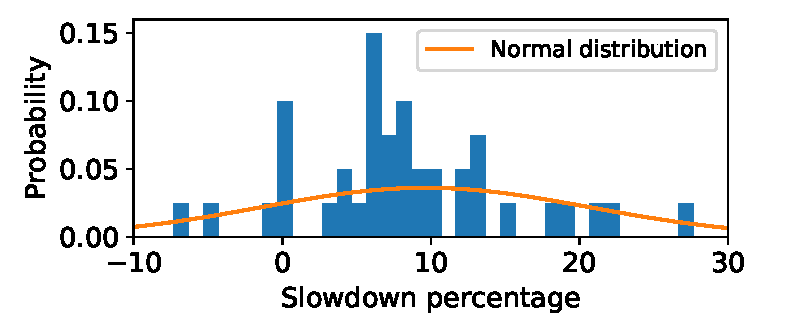
\includegraphics[scale=0.5]{results/density_histogram_filter_slowdown_wordpress_small.pdf}
	\caption{Density histogram of network filter slowdown for WordPress sites.}
	\label{fig:histogram_slowdown_wordpress}
\end{figure}
\fi

Finally, we report the string verification time as a function of its length, for the WordPress sites, shown in \autoref{fig:verification_time_string_length_wordpress}. The Spearman's rank correlation for this set of data is 0.630.


\begin{figure}[h]
	\begin{center}
	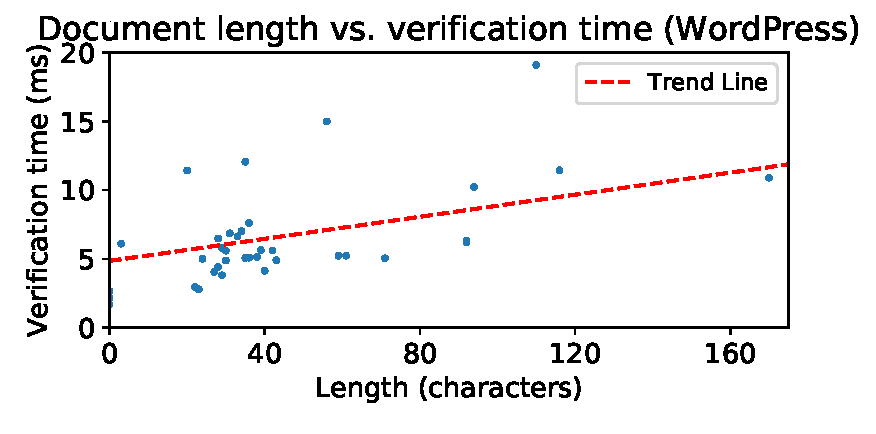
\includegraphics[scale=0.55]{results/string_length_vs_verification_time_wordpress_small.pdf}
	
	\caption{Scatter plot of network filter time as a function of character length for WordPress sites.}
	\label{fig:verification_time_string_length_wordpress}
\end{center}
\end{figure}




%% %%%%%%%%%%%%%%%%%%%%%%%%%%%%%%%%%%%%%%%%%%%%%%%%%%%%%%%%%%%%%%%%%%%%%%%%
%% \section{Signature Language Specification} \label{appendix:language_specification}
%% %%%%%%%%%%%%%%%%%%%%%%%%%%%%%%%%%%%%%%%%%%%%%%%%%%%%%%%%%%%%%%%%%%%%%%%%

%% We provide a description of our signature language, in particular in the context of WordPress:
%% \begin{itemize}
%% 	\item
%% 	url: If the exploit occurs in a specific URL or subdomain, this is defined as a string, e.g.
%% 	\url{/wp-admin/options-general.php?page=relevanssi\%2Frelevanssi.php}, otherwise null.
%% 	\item
%% 	software: The software framework the page is running if any, e.g. WordPress. A hand-crafted page
%% 	might not have any identifiable software.
%% 	\item
%% 	softwareDetails: If running any software, this provides further information about when to load a signature. For WordPress, these are plugin names as depicted in the HTML of a page running such plugin.
%% 	\item
%% 	version: The version number of the software/plugin/page. This is used for versioning of the software run by the page, as described in \autoref{versioning}.
%% 	\item 
%% 	type: A string describing the signature type. A value of "string" describes a basic signature. A value of 'listener' describes a signature which requires an additional listener in the background page for network requests.
%% 	\item 
%% 	sanitizer: A string with one of the following values: "DOMPurify", "escape", and "regex". This item is optional, the default is DOMPurify.
%% 	\item
%% 	config: The config parameters to go along with the chosen sanitizer, if necessary. For "DOMPurify", the accepted values are as defined by the DOMPurify API (i.e, DOMPurify.sanitize(dirty, config). For "escape", an additional escaping pattern can be provided. For "regex", this should be the pattern to match with the injection point content.
%% 	\item
%% 	typeDet: A string with the following pattern: 'occurrence-uniqueness'. As described in Section 2.4, this specifies whether there are several injection points in the HTML.
%% 	\item
%% 	endPoints: An array of startpoint and endpoint tuples.
%% 	\item 
%% 	endPointsPositions: An array of integer tuples. These are optional but useful when the one of the endPoints HTML are used throughout the whole page and appear a fixed number of times. For example: if an injection ending point happens on an element <h3 class='my-header'>, this element might have 10 appearances throughout the page. However, only the 4th is an injection ending point. The signature would specify the second element of the tuple to be 7, as it would be the 7th such item in a regex match array (using 1-based indexing), counting from the bottom up. For ending points, we have to count from the bottom up because the attacker can inject arbitrarily many of these elements before it, and vice versa for starting points.
%% \end{itemize}

%% Additionally, if the value of type is `listener', the signature will have an additional field called listenerData. Similarly to a regular signature, this consists of the following pieces of information:
%% \begin{itemize}
%% 	\item 
%% 	listenerType: The type of network listener as defined by the WebRequest API (e.g. `script', `XHR', etc.)
%% 	\item
%% 	listenerMethod: The request's HTTP method, for example "GET" or "POST".
%% 	\item
%% 	url: the URL of the request target.
%% \end{itemize}

	\bibliographystyle{IEEEtran}
	\bibliography{references}

\end{document}
